\begin{frame}{lattice constant and k-grid study part 1}
	\begin{columns}
		\begin{column}{0.48\linewidth}
			\centering
			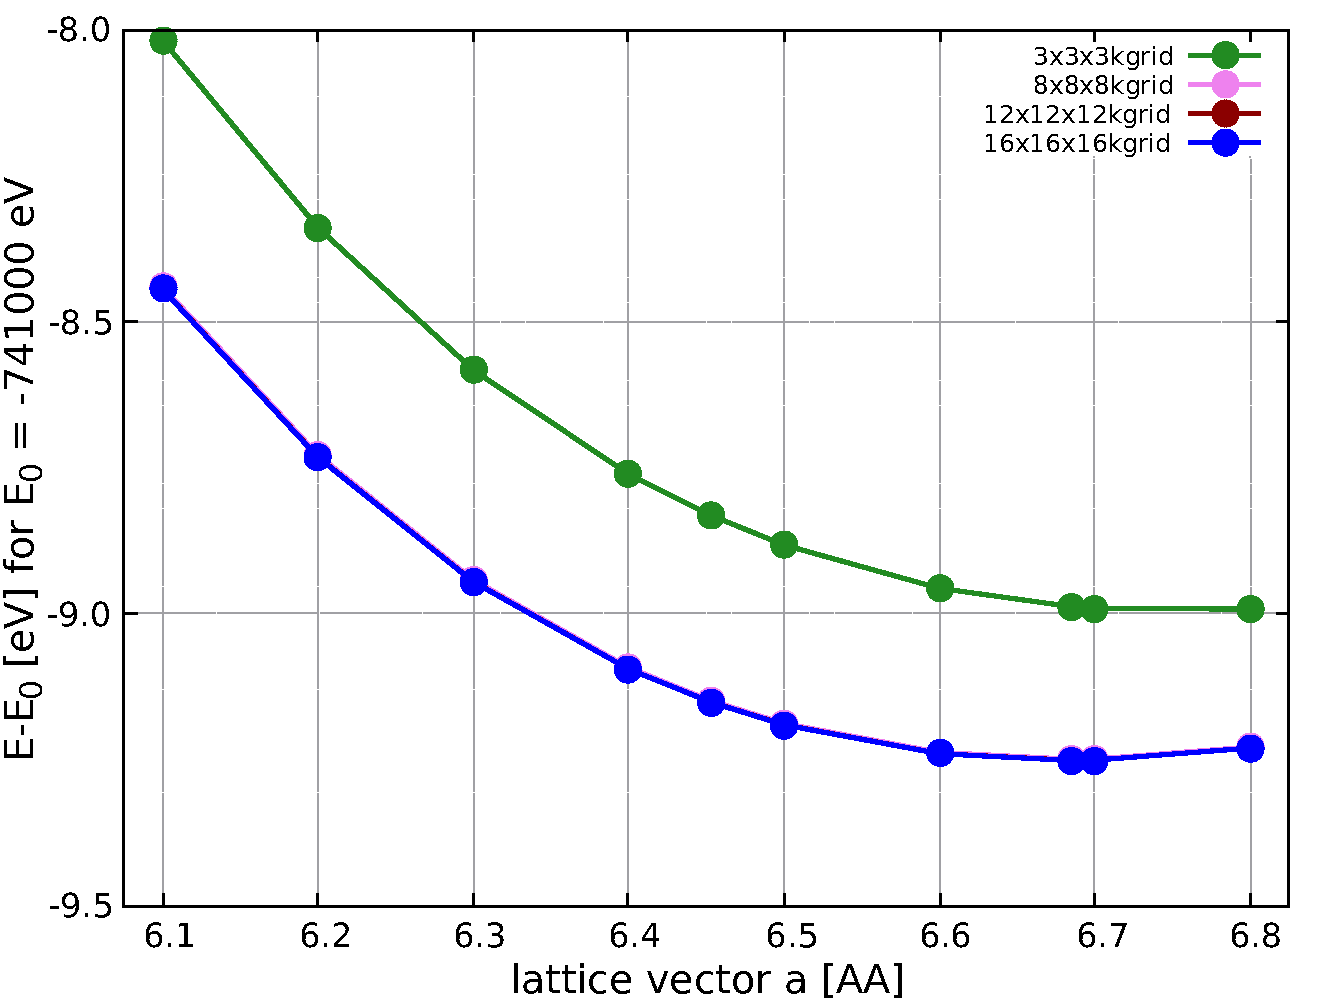
\includegraphics[width=\linewidth]{andere_bilder/plot_energies_hgte_bulk_all_kgrid_in_one.pdf}
			\\
			Lattice constant $a$ with respect to the total energy, calculated with 4 different k-grids. 
		\end{column}
		\begin{column}{0.48\linewidth}
			\centering
			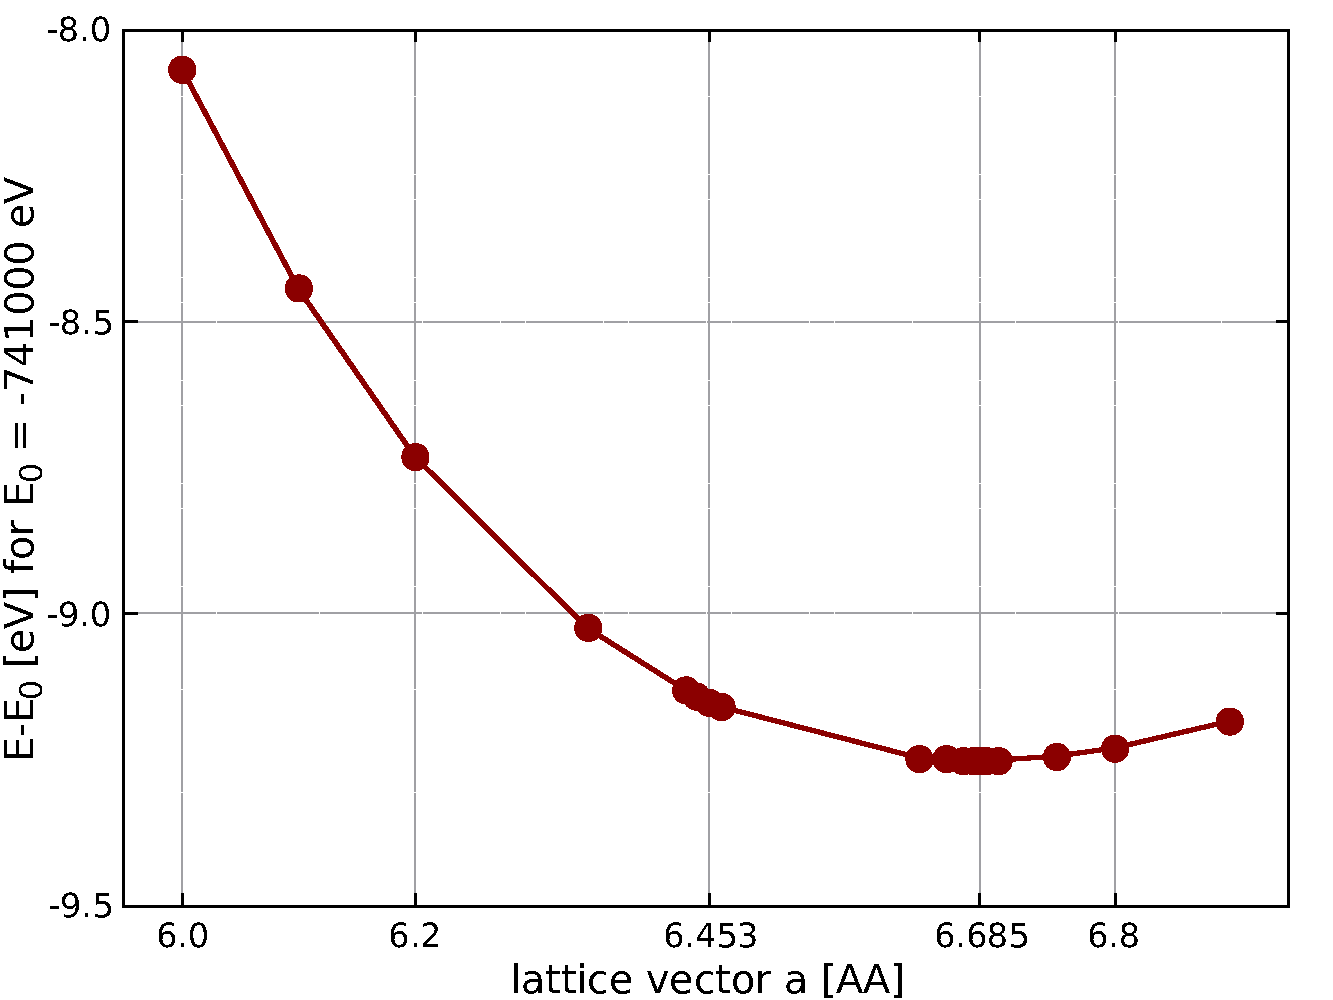
\includegraphics[width=\linewidth]{andere_bilder/lattice_constant_study_spin_none_no_soc.pdf}
			\\
			Lattice constant $a$ with respect to the total energy. The lowest energy was found for 6.685\,$\unit{\AA}$. %\vspace{12.5pt}
		\end{column}
	\end{columns}
	\note{ Let's now turn to the results. First of all I like to mention, that the input data for calculations performed by FHI-aims are the geometry.in and the control.in. The geometry.in contains the coordinates of the lattice vectors and of the atoms. The control.in contains physical settings like the exchange-correlation method, the spin treatment and the relativistic effects. It also contains convergence criteria of the self convergence cycle, the k-grid settings and Informations about all atomic species represented in the geometry.in. \\
	Before starting the calculations for the band structure, it is recommended to do a
	lattice constant study and a k-grid study. So let's have a look at the plot at the left. Here we see the lattice constant with respect to the total energy of the bulk calculated with different k-grids. As we can see the k-grid 3 3 3 gives no good results. The plots for 8 to 16 kgrid overlays, so 8x8x8 seems to be enough to bring physically correct results. In the right picture we see the lattice constant plot for one specific kgrid configuration. The energetically most stable constitution of a crystal structure is given by the lattice constant $a$ with the smallest total system energy, in this case, I found 6.685 Angström for the lowest energy.}
\end{frame}

\begin{frame}{lattice constant and k-grid study part 2}
	\scriptsize{
	Total energy $E [\unit{eV}] - E_0$ (with $E_0$ the energy offset) as a function of k-grid spacing.} \vspace{.1cm}
	\begin{columns}
		\begin{column}{.4\linewidth}
%			\centering
			\scriptsize{
				Bulk: %with $E_0= -741008 \,\unit{eV}$
			}\\ 
			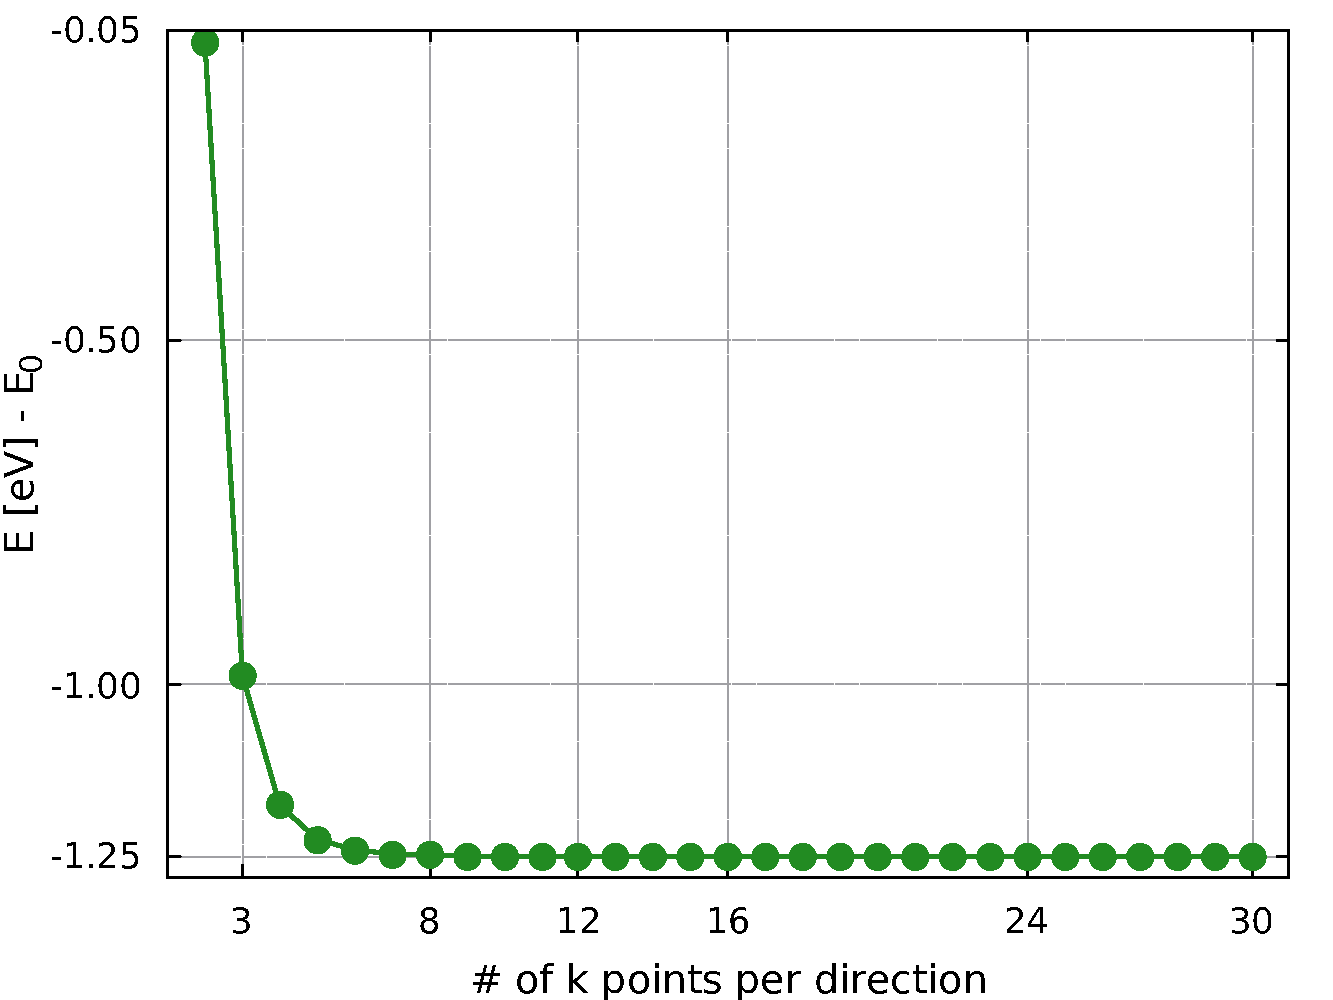
\includegraphics[width=\linewidth]{andere_bilder/kgrid_bulk.pdf}
		\end{column}
		\begin{column}{.4\linewidth}
			\scriptsize{
				Slab with 4 layers: %with $E_0= -1482047 \,\unit{eV}$
			}\\
			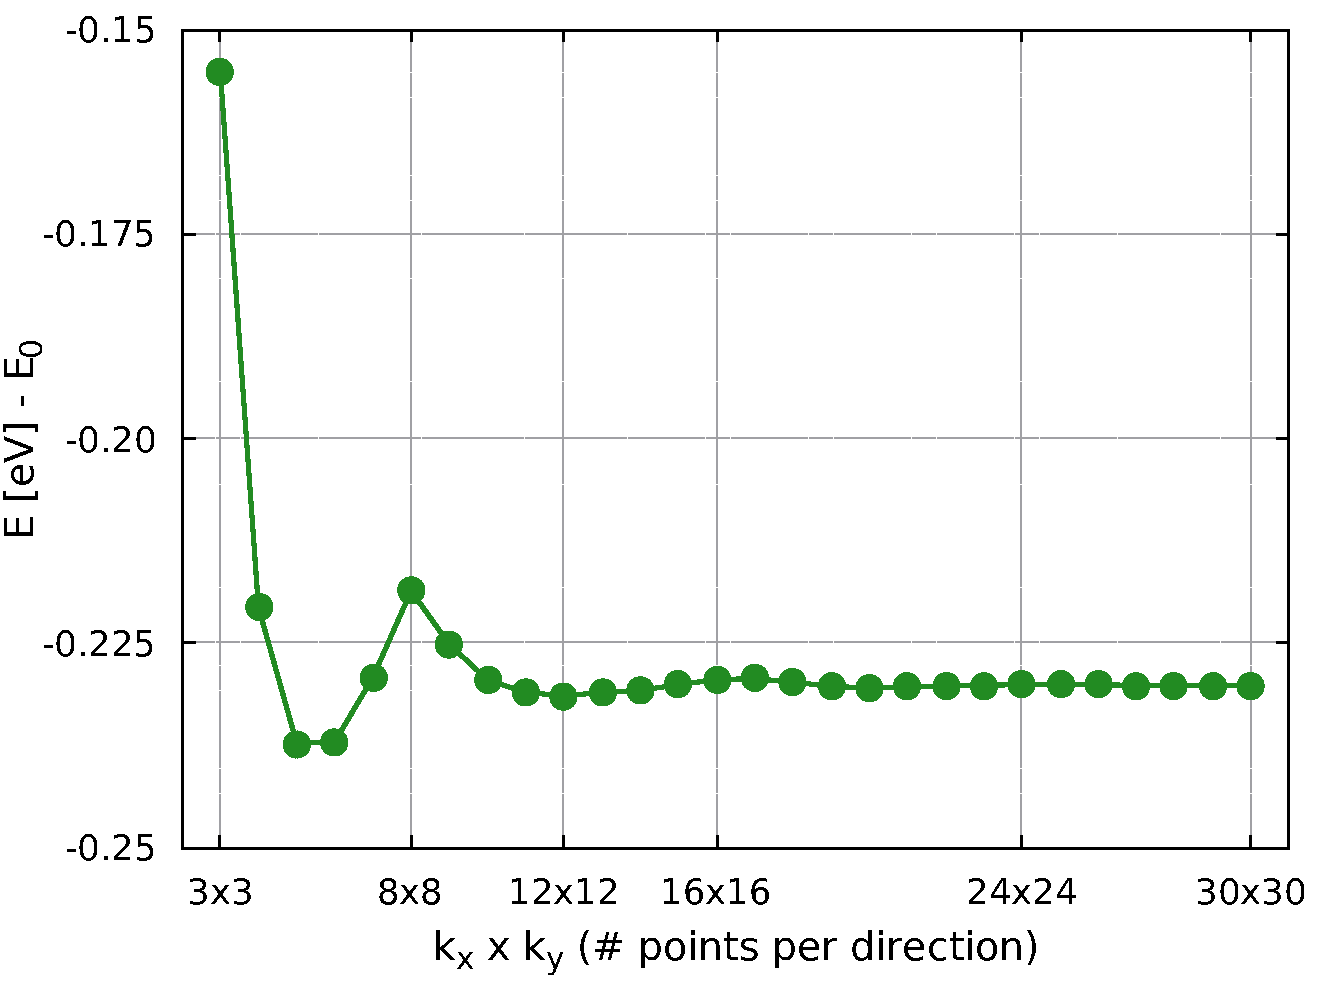
\includegraphics[width=\linewidth]{andere_bilder/kgrid_1x1x4_layers.pdf}
		\end{column}
		\end{columns}
		\begin{columns}
		\begin{column}{.4\linewidth}
			\scriptsize{
				Slab with 8 layers:% with $E_0= -2964065 \,\unit{eV}$
			}\\
			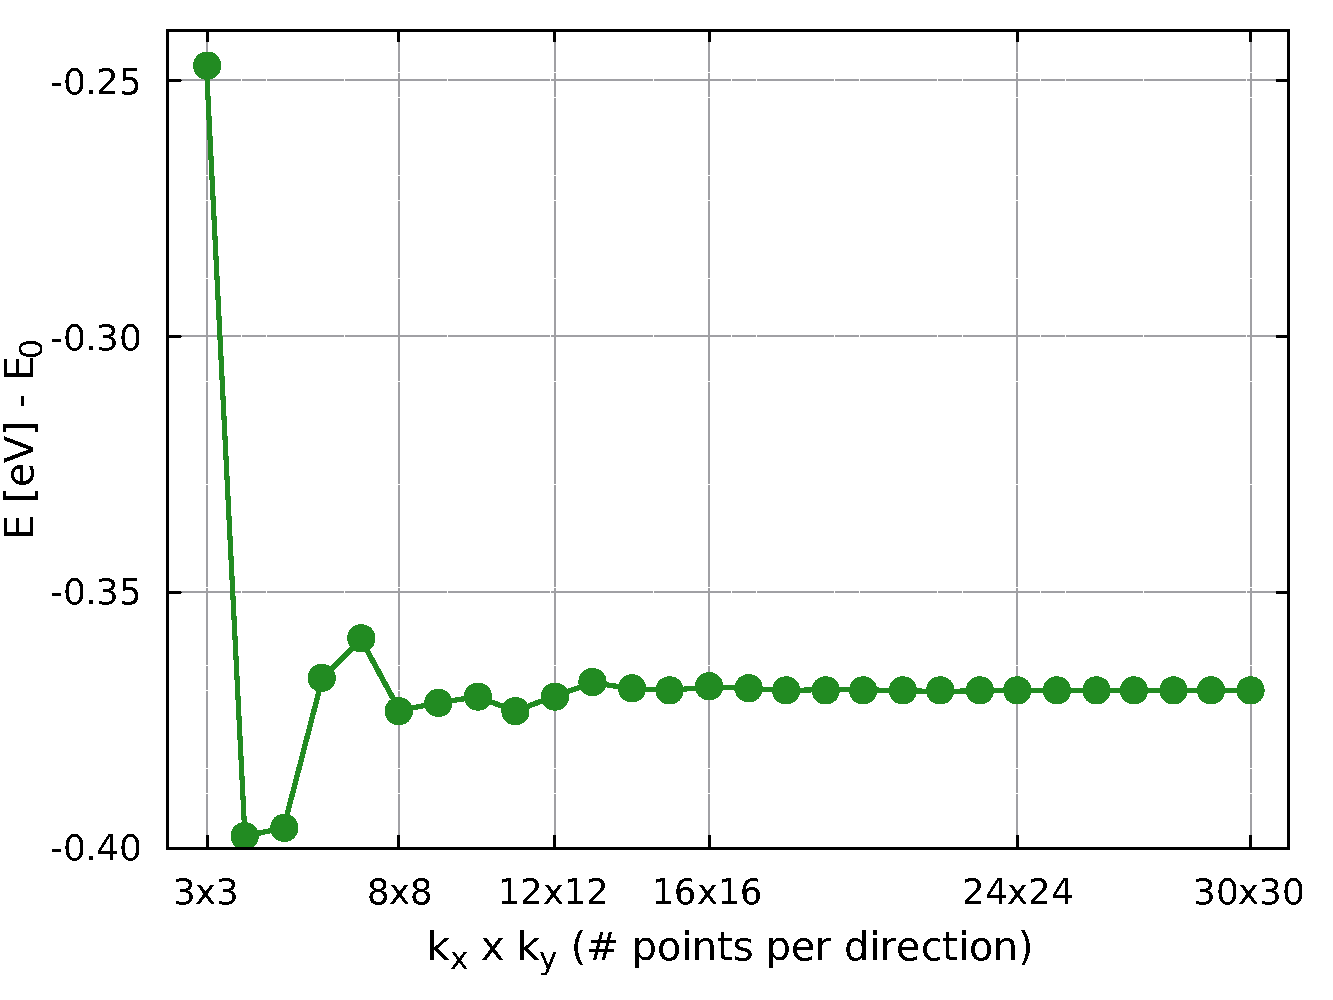
\includegraphics[width=\linewidth]{andere_bilder/kgrid_1x1x8_layers.pdf}
		\end{column}
		\begin{column}{.4\linewidth}
			\scriptsize{
				Slab with 16 layers: %with $E_0= -5928101 \,\unit{eV}$
			} \\
			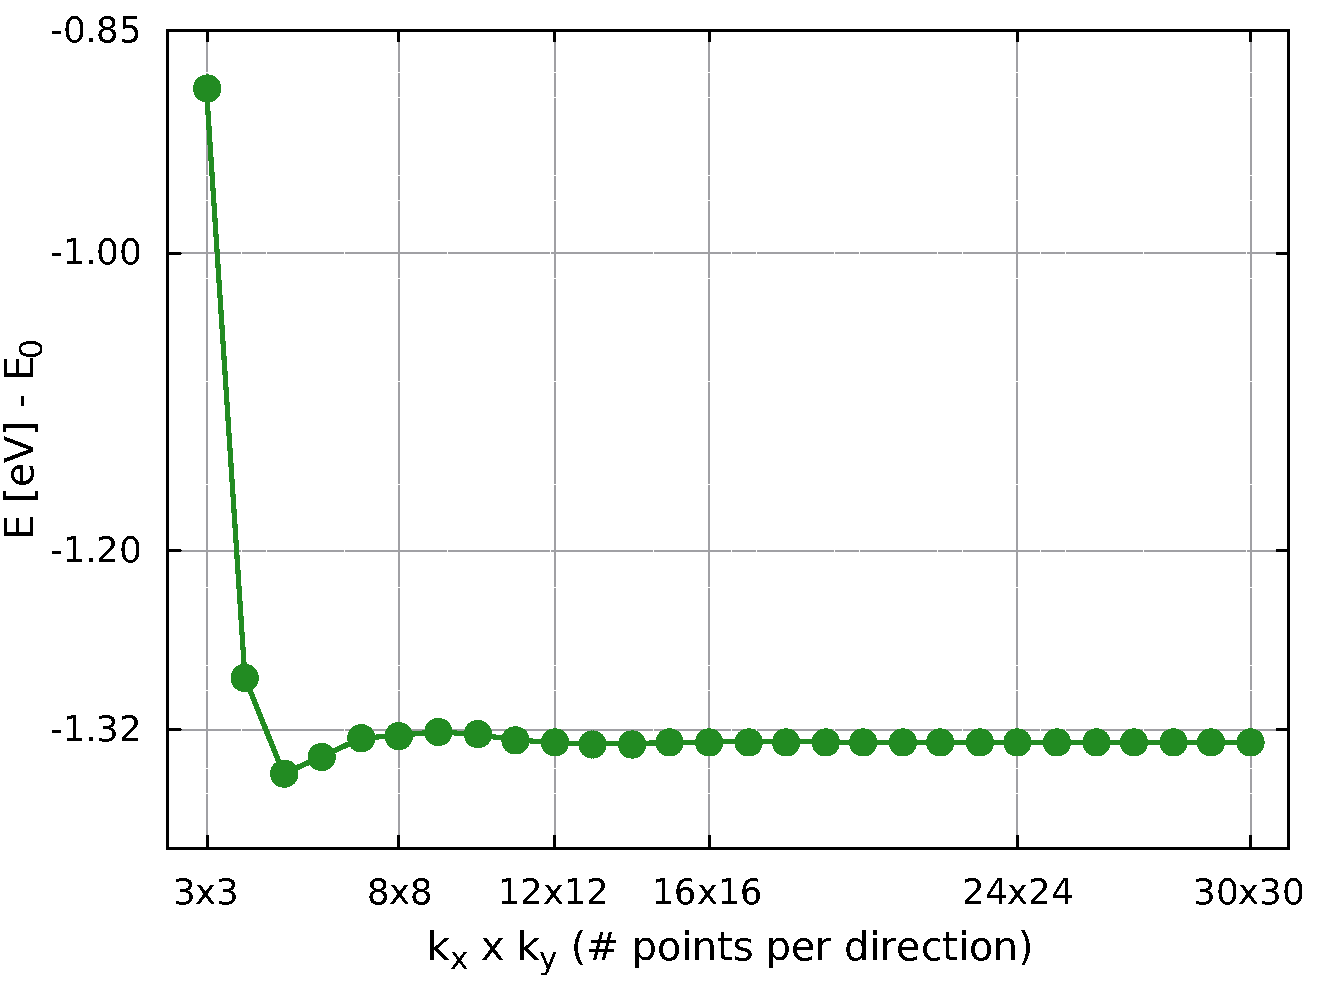
\includegraphics[width=\linewidth]{andere_bilder/kgrid_1x1x16_layers.pdf}
		\end{column}
	\end{columns}
	\note{ This lattice constant then was used for a detailed kgrid study of the bulk and slabs with 4, 8 and 16 layers. Note that for the slabs, k z was set to 1 and that E 0 is just a number different for every plot which was chosen for smaller numbers in the y axis. Since a higher kgrid recommends more computational effort, the most economic kgrid directly after the it has converged to a certain energy. That number was nearly the same for the bulk and the all slabs, namely 12. The oscillation in the plots for the slabs comes from the translation symmetry break in k z direction and therefore it is no wonder that this oscillation becomes smaller for thicker slabs.
	The kgrid used for the following calculations was 24 since higher kgrid gives smoother bands and the additional computational effort was small.}
\end{frame}

\begin{frame}[fragile]{Projected bulk band structure (PBBS)}
	Making 40 slices in 2D Brillouin zone of the bulk from $k_z=0$ to $k_z=k_{z,\text{max}}$ where $k_{z,\text{max}}=\frac{\pi}{a}$. Input example:
	\vspace{-.3cm}
	\begin{columns} 
		\begin{column}<2->{\linewidth}\scriptsize{
			\begin{verbatim}
			output band 0.5   0.0   0.01175   0.0   0.0   0.01175    80  J     Gamma
			output band 0.0   0.0   0.01175   0.5   0.5   0.01175    80  Gamma K
			output band 0.5   0.5   0.01175   0.5   0.0   0.01175    80  K     J
			\end{verbatim} }
		\end{column}
	\end{columns}
	\begin{columns}<3->
		\begin{column}{.165\linewidth} \scriptsize{
				$k_z=0$}
		\end{column} \hspace{-.5cm}
		\begin{column}{.33\linewidth}
%		\begin{figure}[c]{\linewidth}
			\centering
			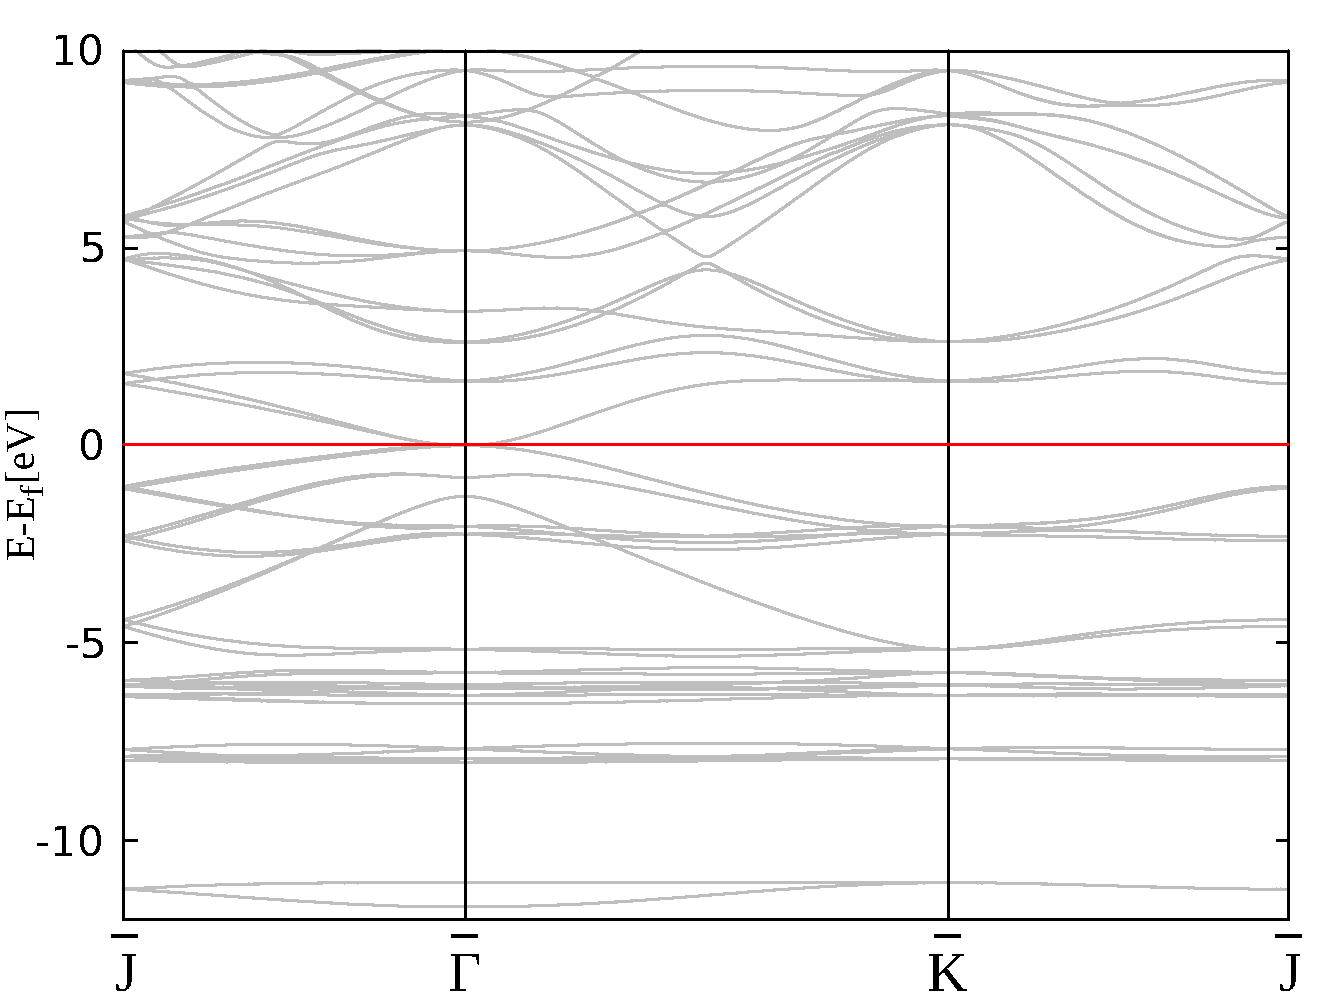
\includegraphics[width=\linewidth]{andere_bilder/0_bulk_-12_10.pdf}
%			\caption{PBBS for $k_z$ is equal to zero.}
%		\end{figure}
		\end{column}
		\begin{column}{.33\linewidth}
%		\begin{figure}[c]{\linewidth}
			\centering
			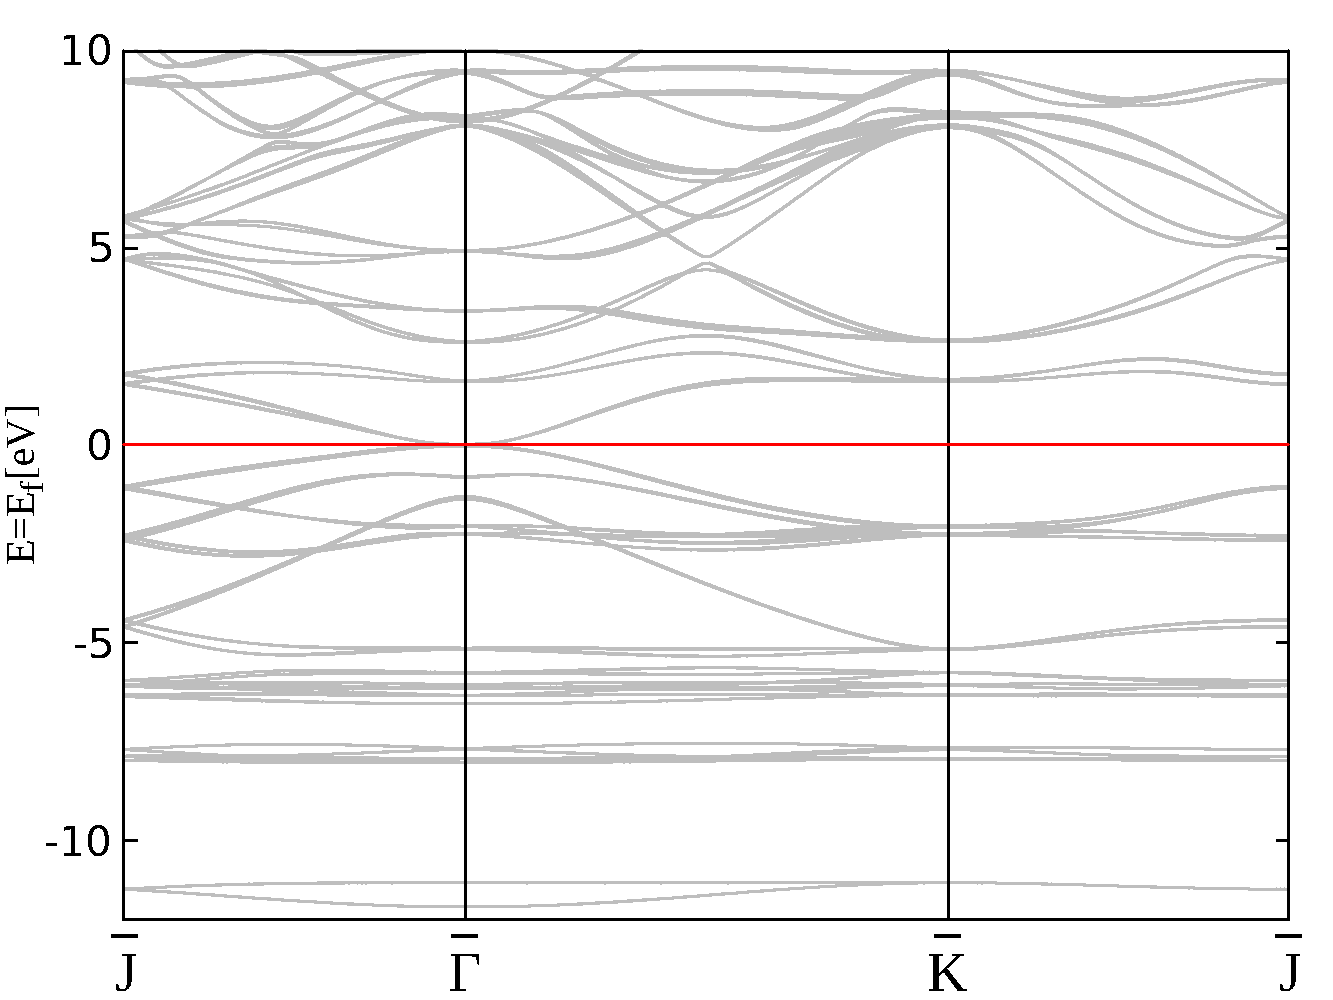
\includegraphics[width=\linewidth]{andere_bilder/4_bulk_-12_10.pdf}
%			\caption{Ensemble for PBBS for $k_z$ having values from 0 to $1/10\cdot k_{z,\text{max}}$}
%		\end{figure}
		\end{column}
		\begin{column}{.165\linewidth} \scriptsize{
			${k_z=0}$ to ${1/10\cdot k_{z,\text{max}}}$ }
		\end{column}
	\end{columns}
	\begin{columns}
		\begin{column}{.165\linewidth} \scriptsize{
				${k_z=0}$ to ${1/4\cdot k_{z,\text{max}}}$ }
		\end{column} \hspace{-.5cm}
		\begin{column}{.33\linewidth}
%		\begin{figure}[c]{\linewidth}
			\centering
			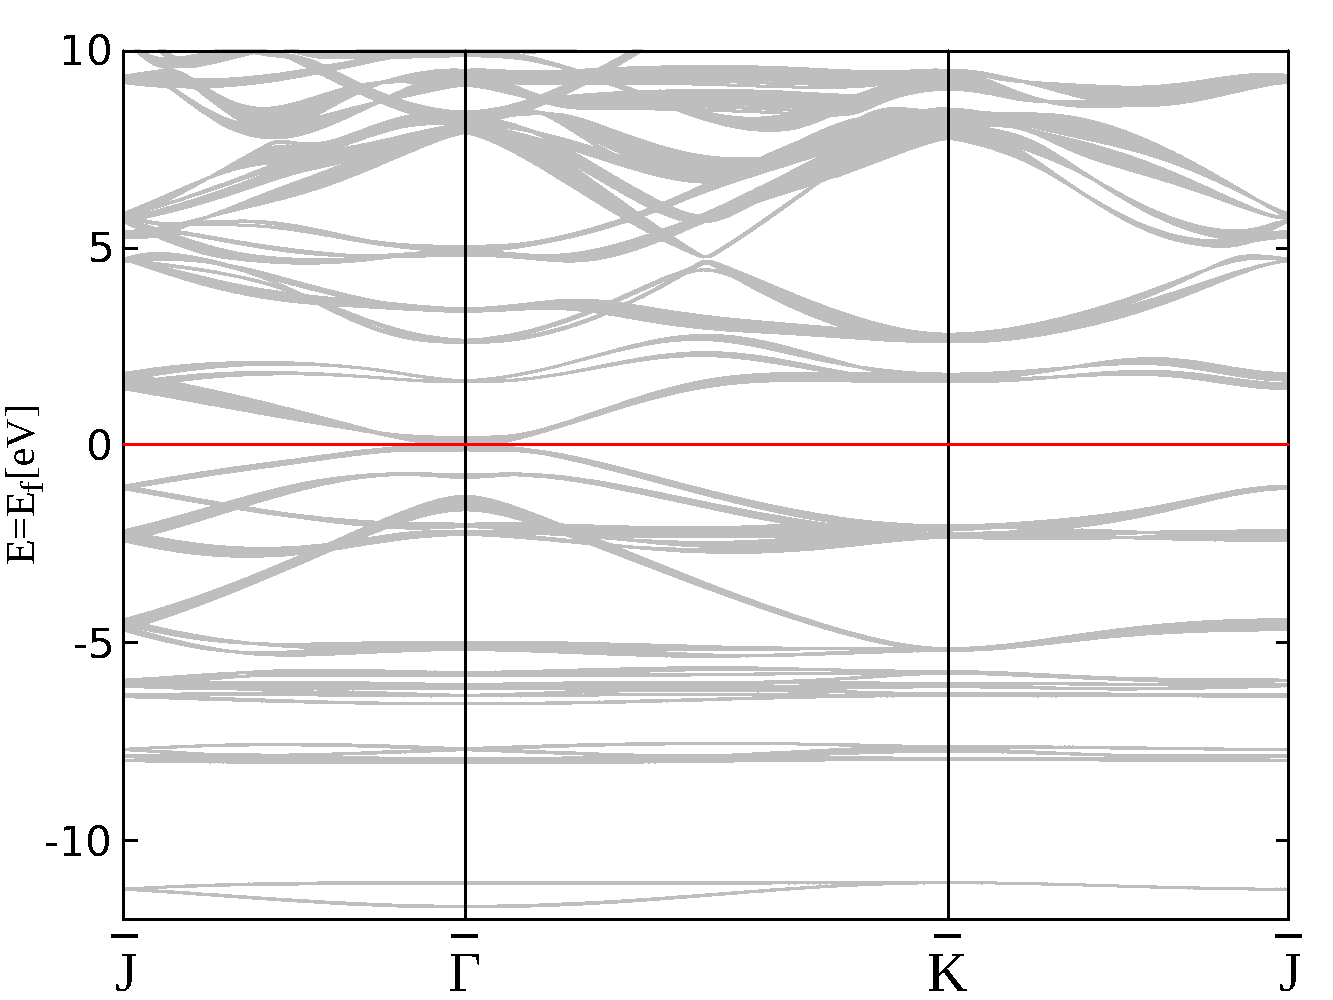
\includegraphics[width=\linewidth]{andere_bilder/10_bulk_-12_10.pdf}
%			\caption{Ensemble for PBBS for $k_z$ having values from 0 to $1/4\cdot k_{z,\text{max}}$} 
%		\end{figure}
		\end{column}
		\begin{column}{.33\linewidth}
%		\begin{figure}[c]{\linewidth}
			\centering 
			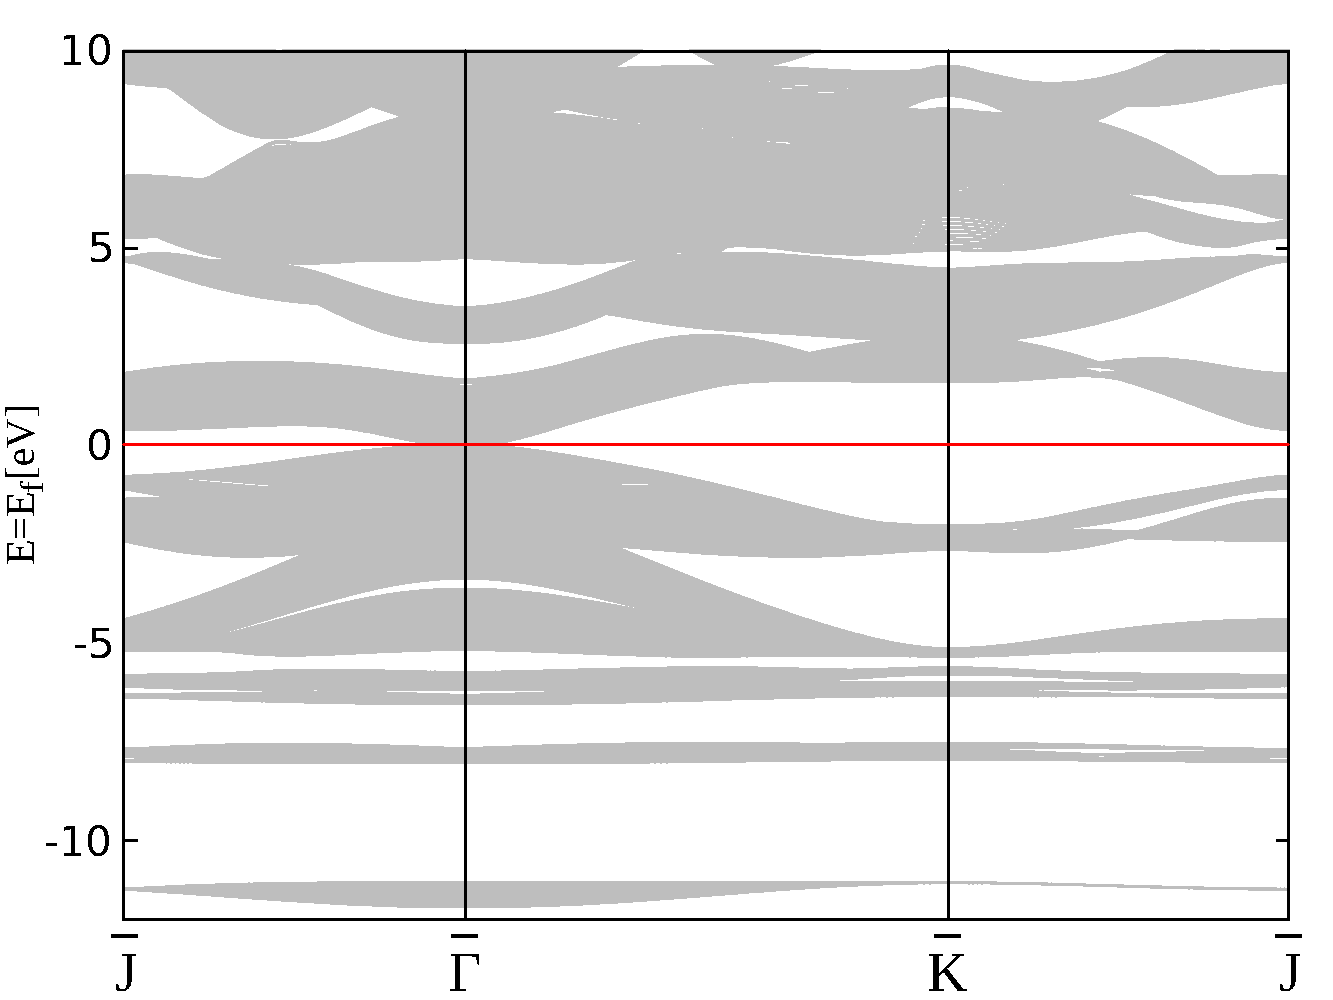
\includegraphics[width=\linewidth]{andere_bilder/bulk_-12_10.pdf}
%			\caption{Whole PBBS for all the values of $k_z$ going from 0 to $k_{z,\text{max}}$} 
%		\end{figure}
		\end{column}
		\begin{column}{.165\linewidth} \scriptsize{
				${k_z=0}$ to $k_{z,\text{max}}$ }
		\end{column}
	\end{columns}	
	\note{
		}
\end{frame}


\begin{frame}{PBBS with 4 and 5 layer slabs}
	\begin{columns}
		\begin{column}{.34\linewidth}
			\centering
			Te-Hg termination
		\end{column}
		\begin{column}{.34\linewidth}
			\centering
			Te-Te termination
		\end{column}
		\begin{column}{.34\linewidth}
			\centering
			Hg-Hg termination
		\end{column}
	\end{columns}
	\begin{columns}
		\begin{column}{.34\linewidth}
			\centering
			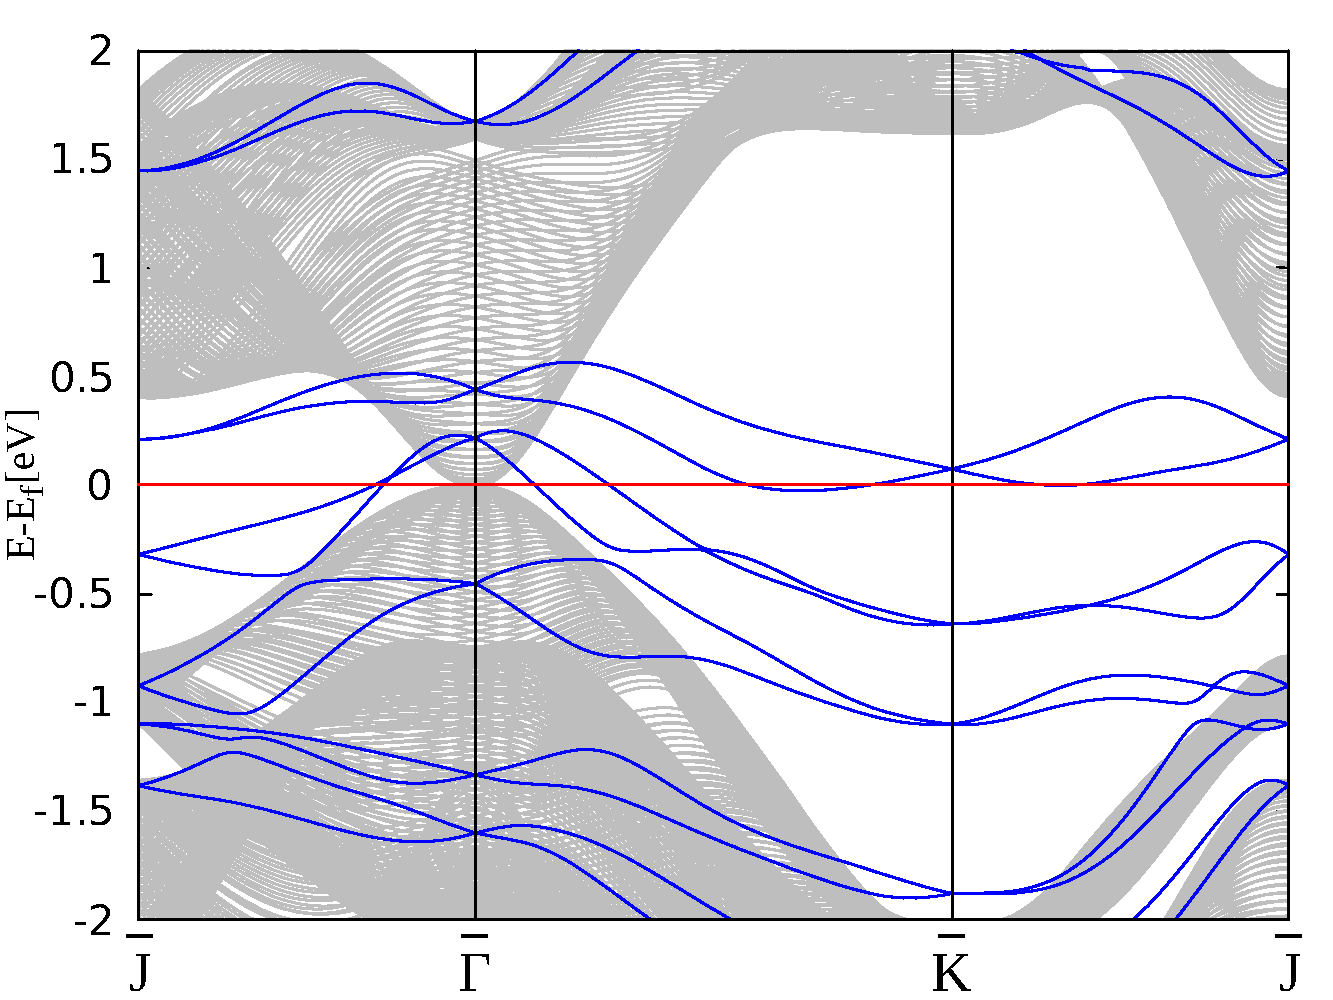
\includegraphics[width=\linewidth]{Te_and_Hg_termination/no_H_bulk+4_layers_no_dos_-2_2.pdf}
%			\caption{4 layers without hydrogens passivating the Te termination}
		\end{column}
		\begin{column}{.34\linewidth}
			\centering
			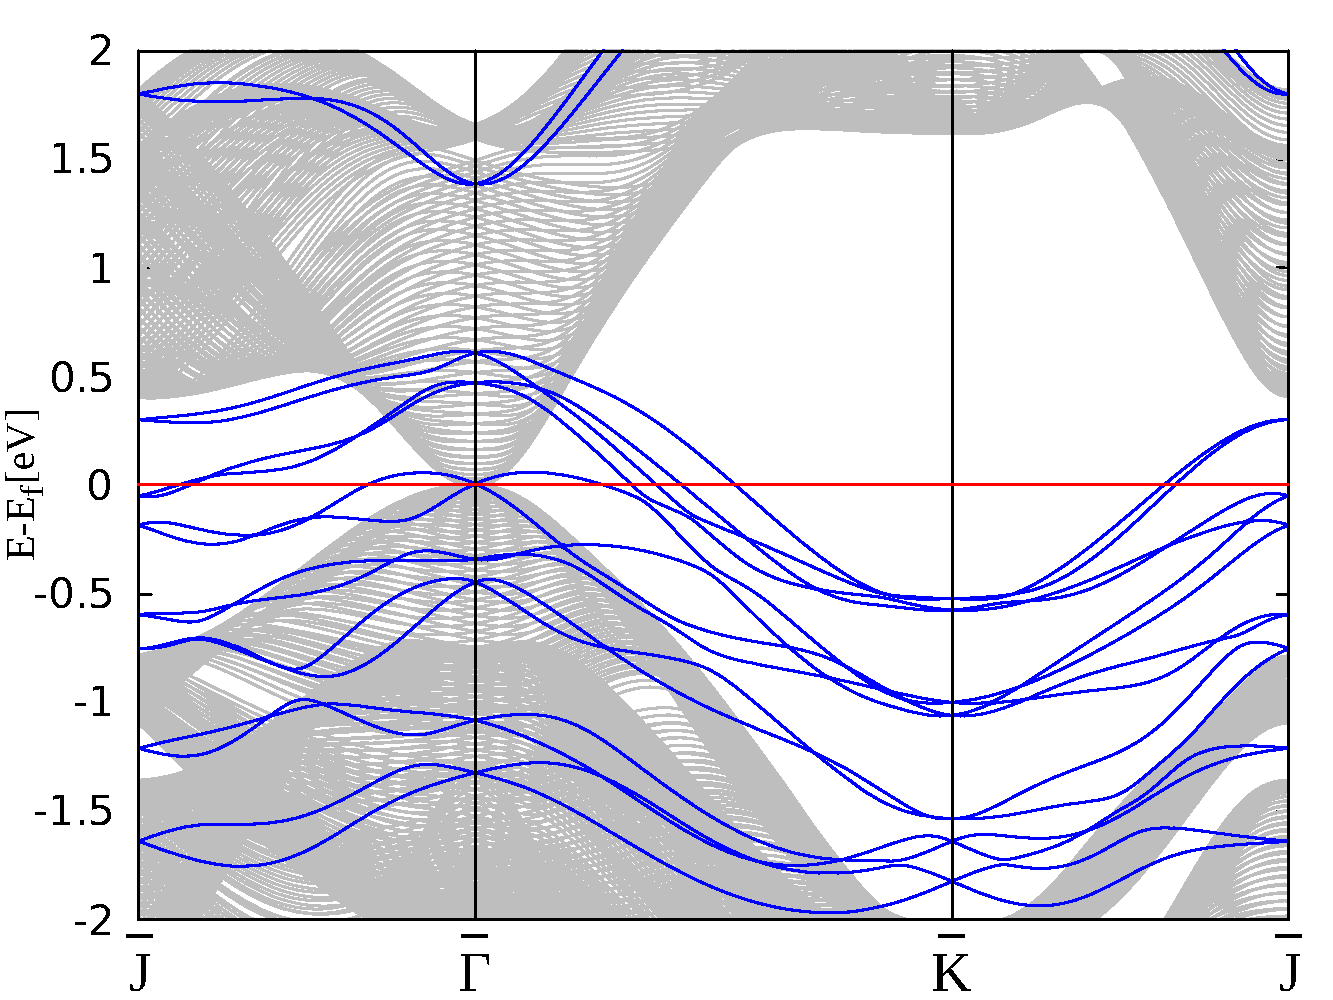
\includegraphics[width=\linewidth]{Te_termination/no_H_bulk+5_layers_no_dos_-2_2.pdf}
%			\caption{5 layers without hydrogens passivating one of the surfaces}
		\end{column}
		\begin{column}{.34\linewidth}
			\centering
			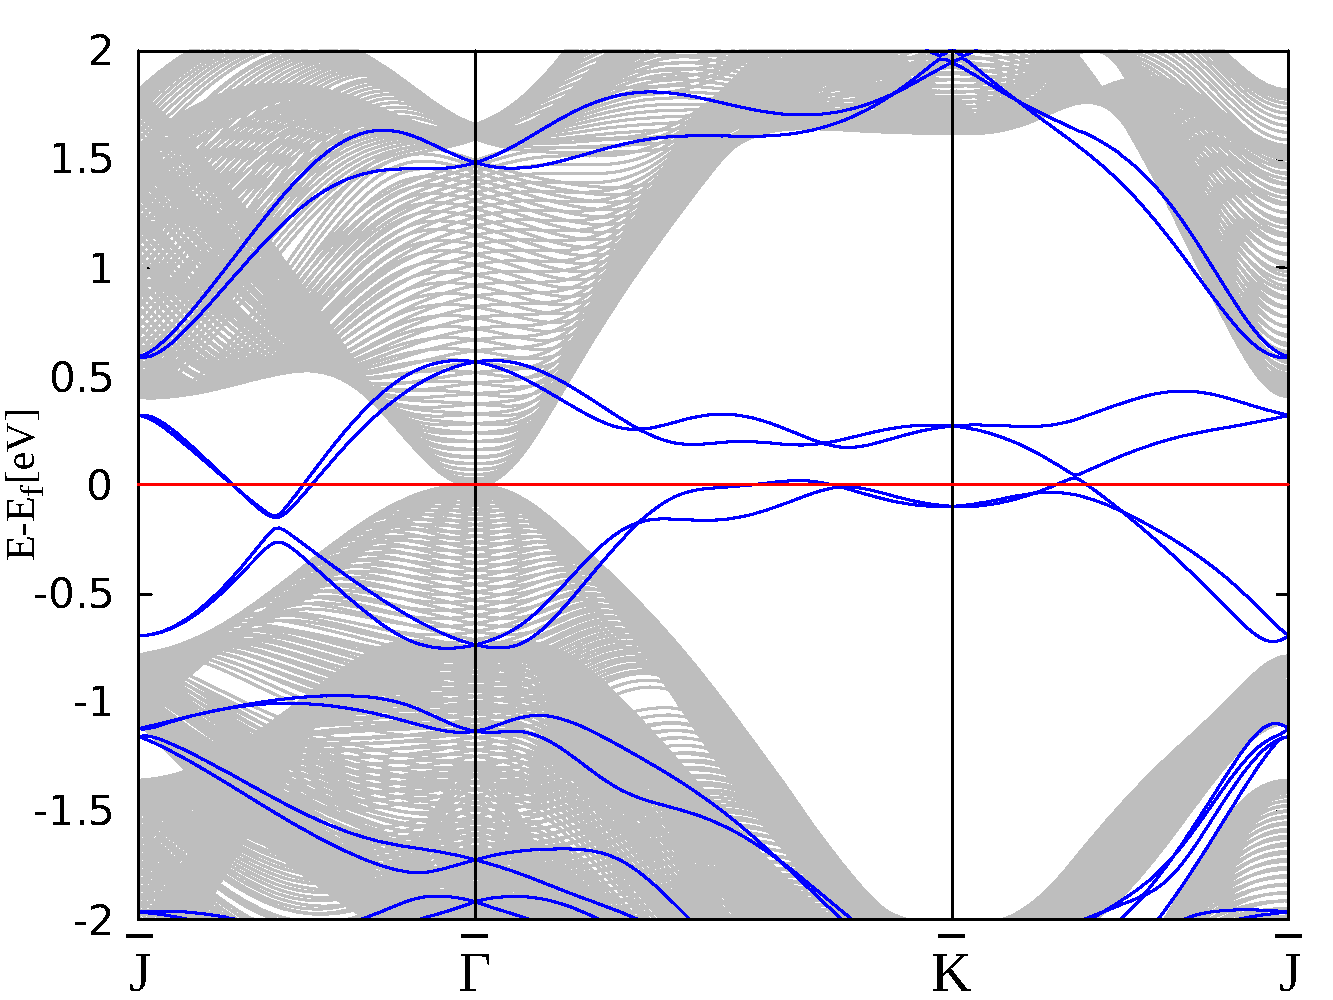
\includegraphics[width=\linewidth]{Hg_termination/no_H_bulk+5_layers_no_dos_-2_2.pdf}
%			\caption{5 layers without hydrogens passivating one of the surfaces}
		\end{column}
	\end{columns}
	\begin{columns}
		\begin{column}{.34\linewidth}
			\centering
			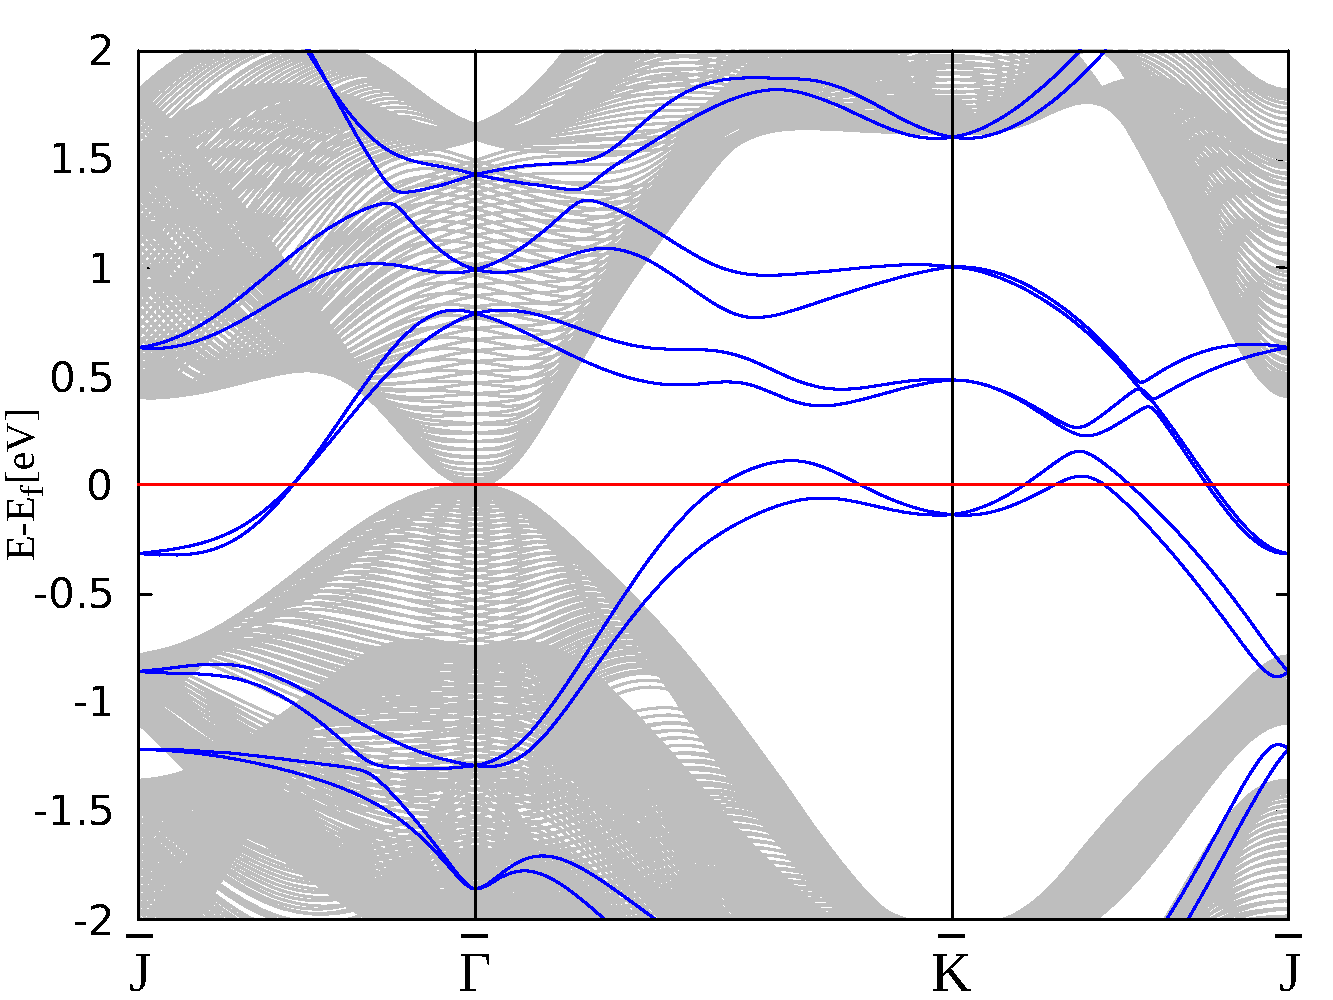
\includegraphics[width=\linewidth]{Te_and_Hg_termination/bulk+4_layers_no_dos_-2_2.pdf}
%			\caption{4 layers with hydrogens on the bottom passivating the Te surface terminations}
		\end{column}
		\begin{column}{.34\linewidth}
			\centering
			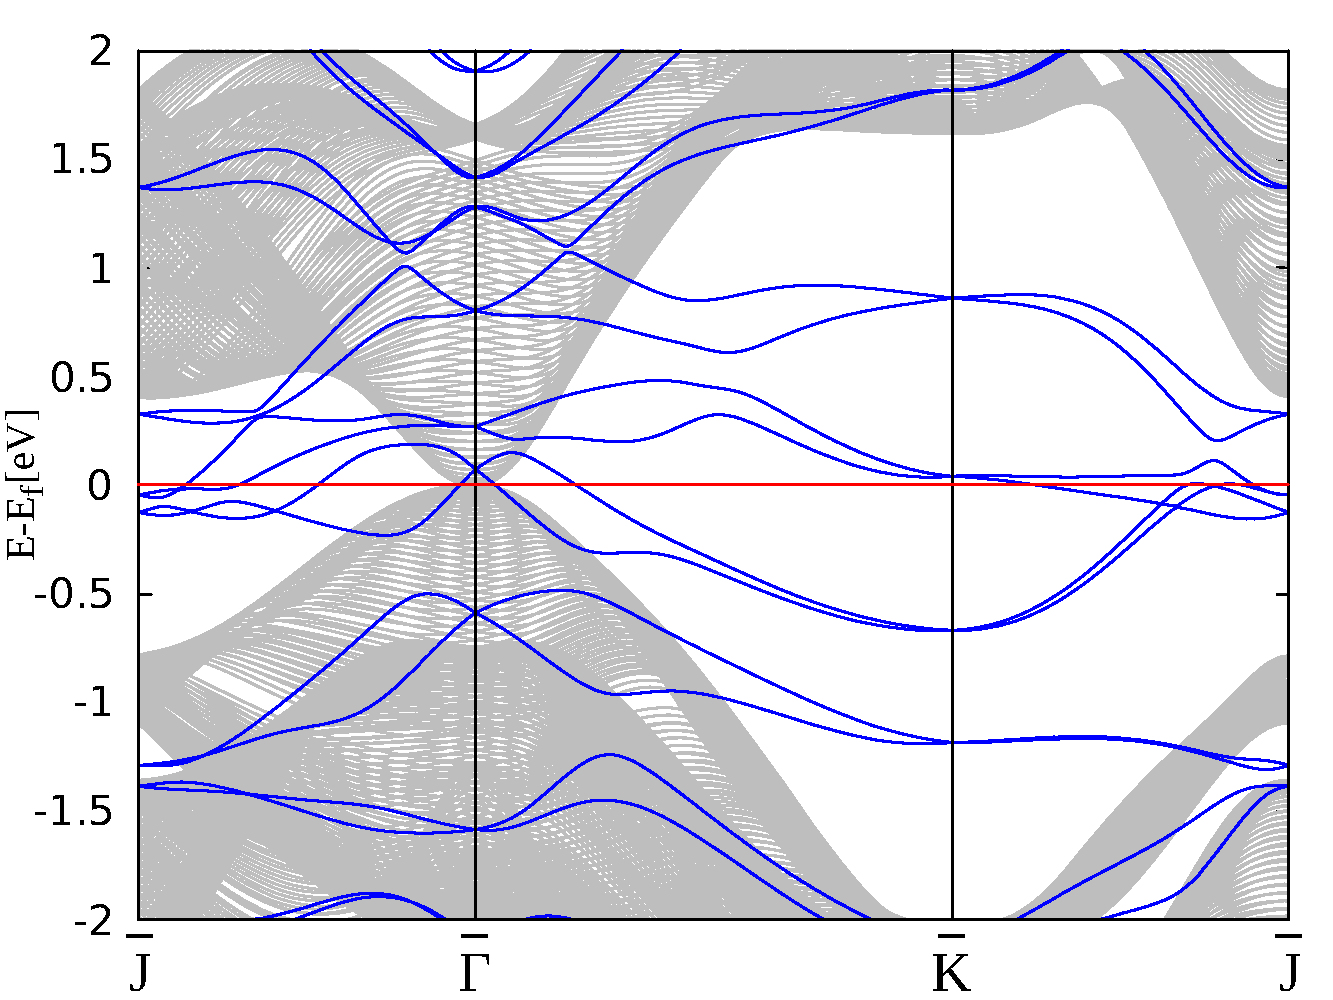
\includegraphics[width=\linewidth]{Te_termination/bulk+5_layers_no_dos_-2_2.pdf}
%			\caption{5 layers with hydrogens on the bottom passivating one of the Te surface terminations}
		\end{column}
		\begin{column}{.34\linewidth}
			\centering
			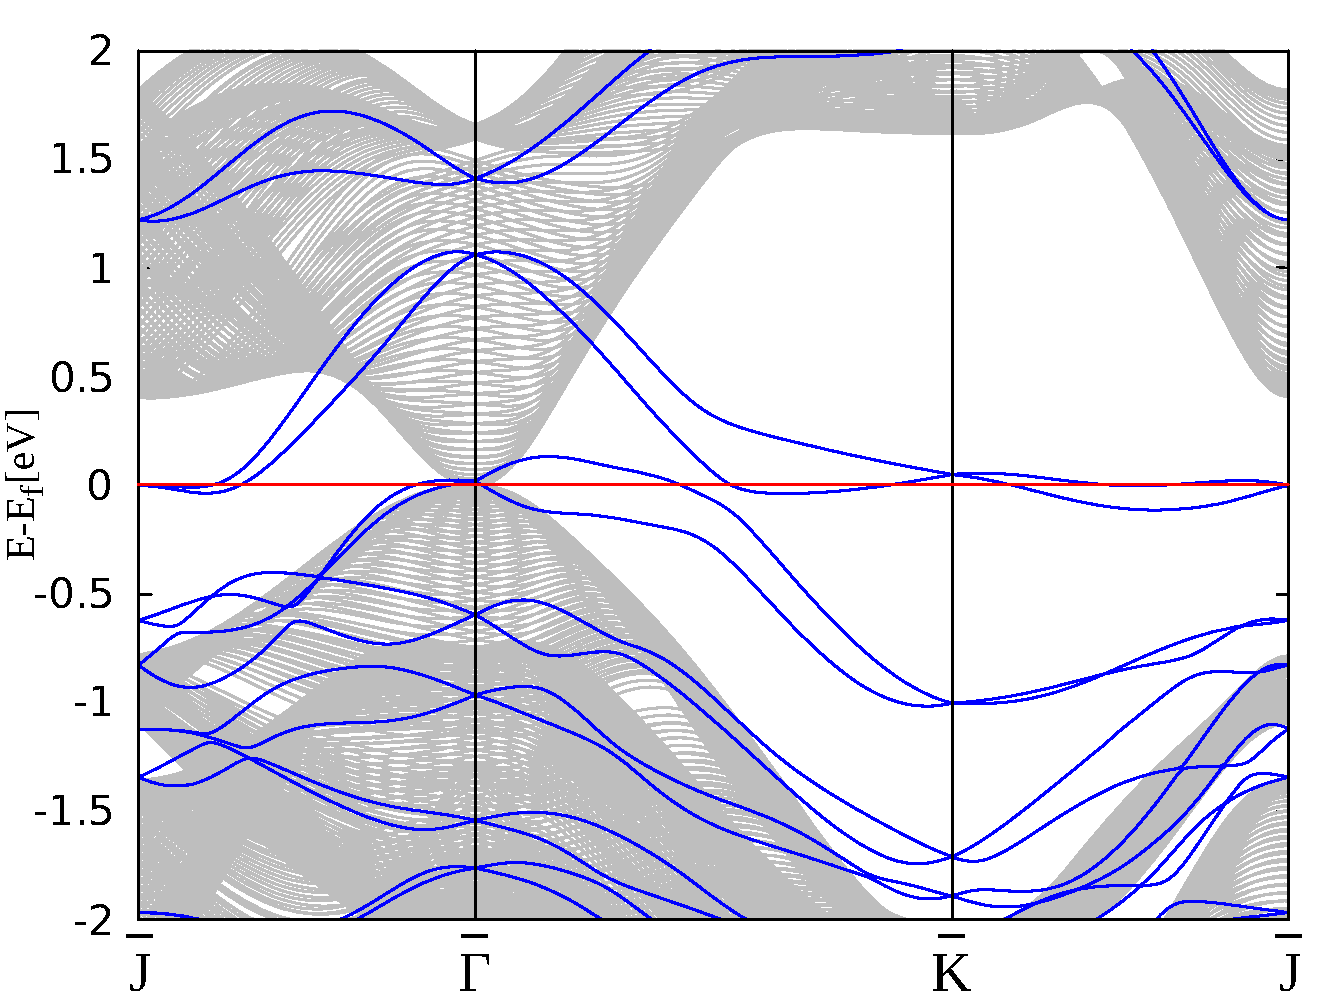
\includegraphics[width=\linewidth]{Hg_termination/bulk+5_layers_no_dos_-2_2.pdf}
%			\caption{5 layers with hydrogens on the bottom passivating one of the Hg surface terminations}
		\end{column}
	\end{columns}
	\vspace{.3cm}
	\footnotesize{
	First row: without hydrogens. \\Second row: with hydrogens passivating one surface.}
\end{frame}

\begin{frame}{PBBS with 8 and 9 layer slabs}
	\begin{columns}
		\begin{column}{.34\linewidth}
			\centering
			Te-Hg termination
		\end{column}
		\begin{column}{.34\linewidth}
			\centering
			Te-Te termination
		\end{column}
		\begin{column}{.34\linewidth}
			\centering
			Hg-Hg termination
		\end{column}
	\end{columns}
	\begin{columns}
		\begin{column}{.34\linewidth}
			\centering
			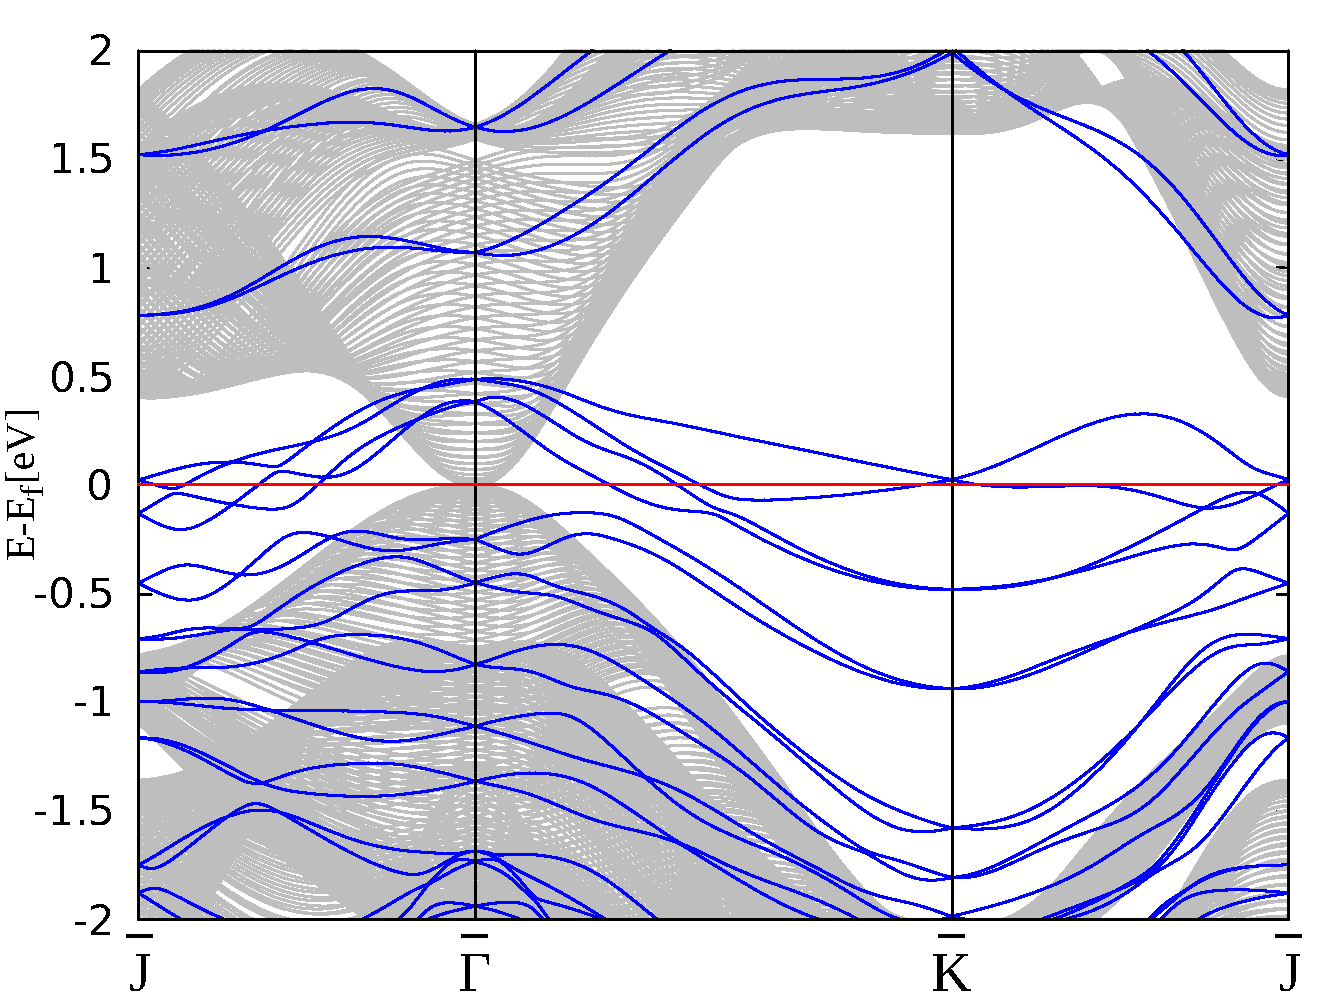
\includegraphics[width=\linewidth]{Te_and_Hg_termination/no_H_bulk+8_layers_no_dos_-2_2.pdf}
%			\caption{8 layers without hydrogens passivating the Te termination}
		\end{column}
		\begin{column}{.34\linewidth}
			\centering
			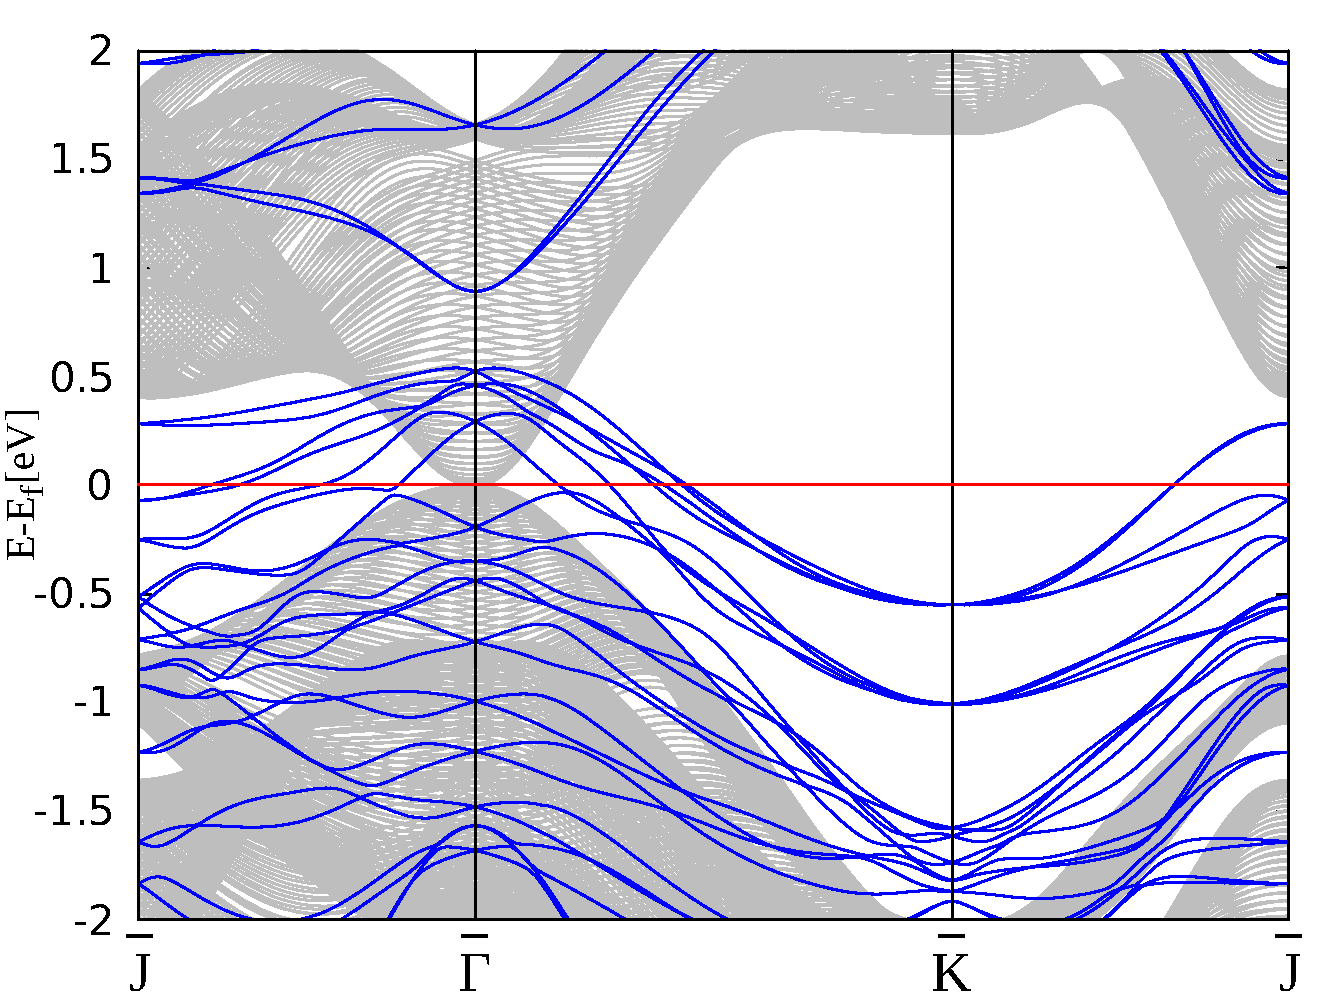
\includegraphics[width=\linewidth]{Te_termination/no_H_bulk+9_layers_no_dos_-2_2.pdf}
%			\caption{9 layers without hydrogens passivating one of the surfaces}
		\end{column}
		\begin{column}{.34\linewidth}
			\centering
			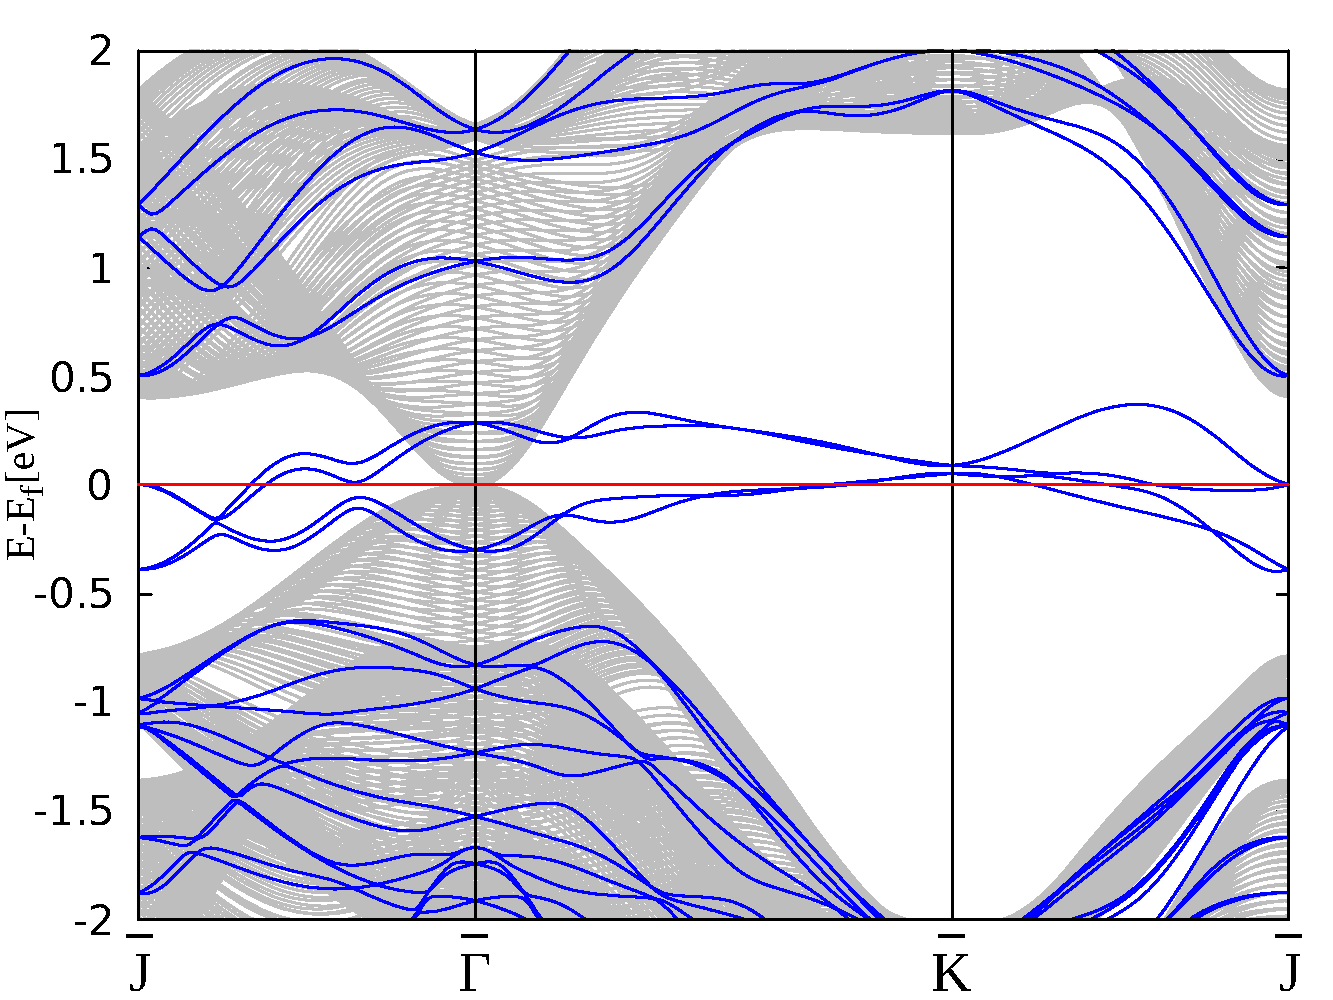
\includegraphics[width=\linewidth]{Hg_termination/no_H_bulk+9_layers_no_dos_-2_2.pdf}
%			\caption{9 layers without hydrogens passivating one of the surfaces}
		\end{column}
	\end{columns}
	\begin{columns}
		\begin{column}{.34\linewidth}
			\centering
			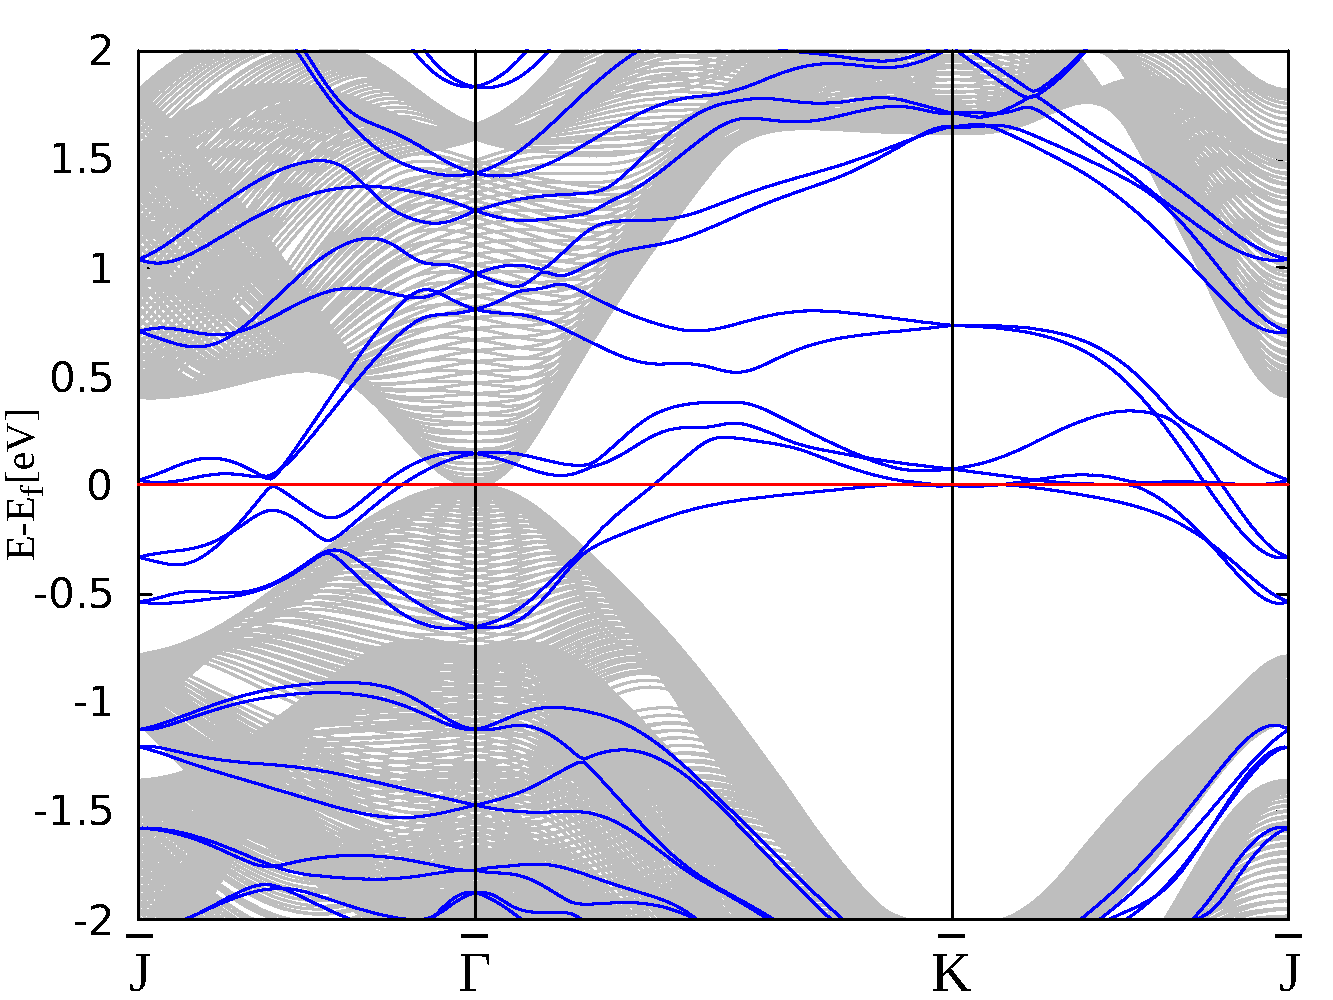
\includegraphics[width=\linewidth]{Te_and_Hg_termination/bulk+8_layers_no_dos_-2_2.pdf}
%			\caption{8 layers with hydrogens on the bottom passivating the Te surface terminations}
		\end{column}
		\begin{column}{.34\linewidth}
			\centering
			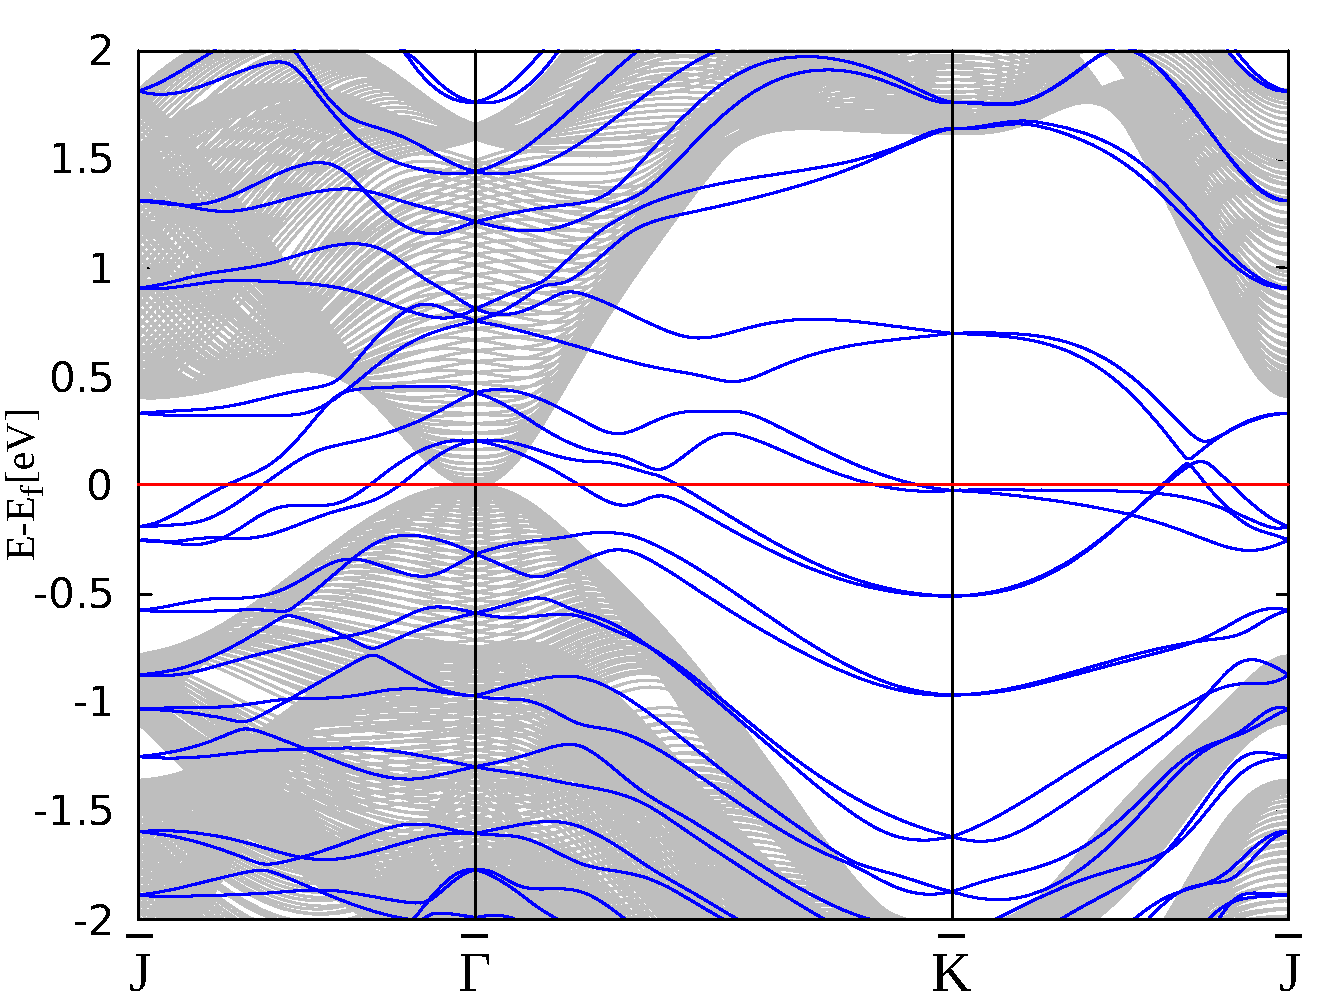
\includegraphics[width=\linewidth]{Te_termination/bulk+9_layers_no_dos_-2_2.pdf}
%			\caption{9 layers with hydrogens on the bottom passivating one of the Te surface terminations}
		\end{column}
		\begin{column}{.34\linewidth}
			\centering
			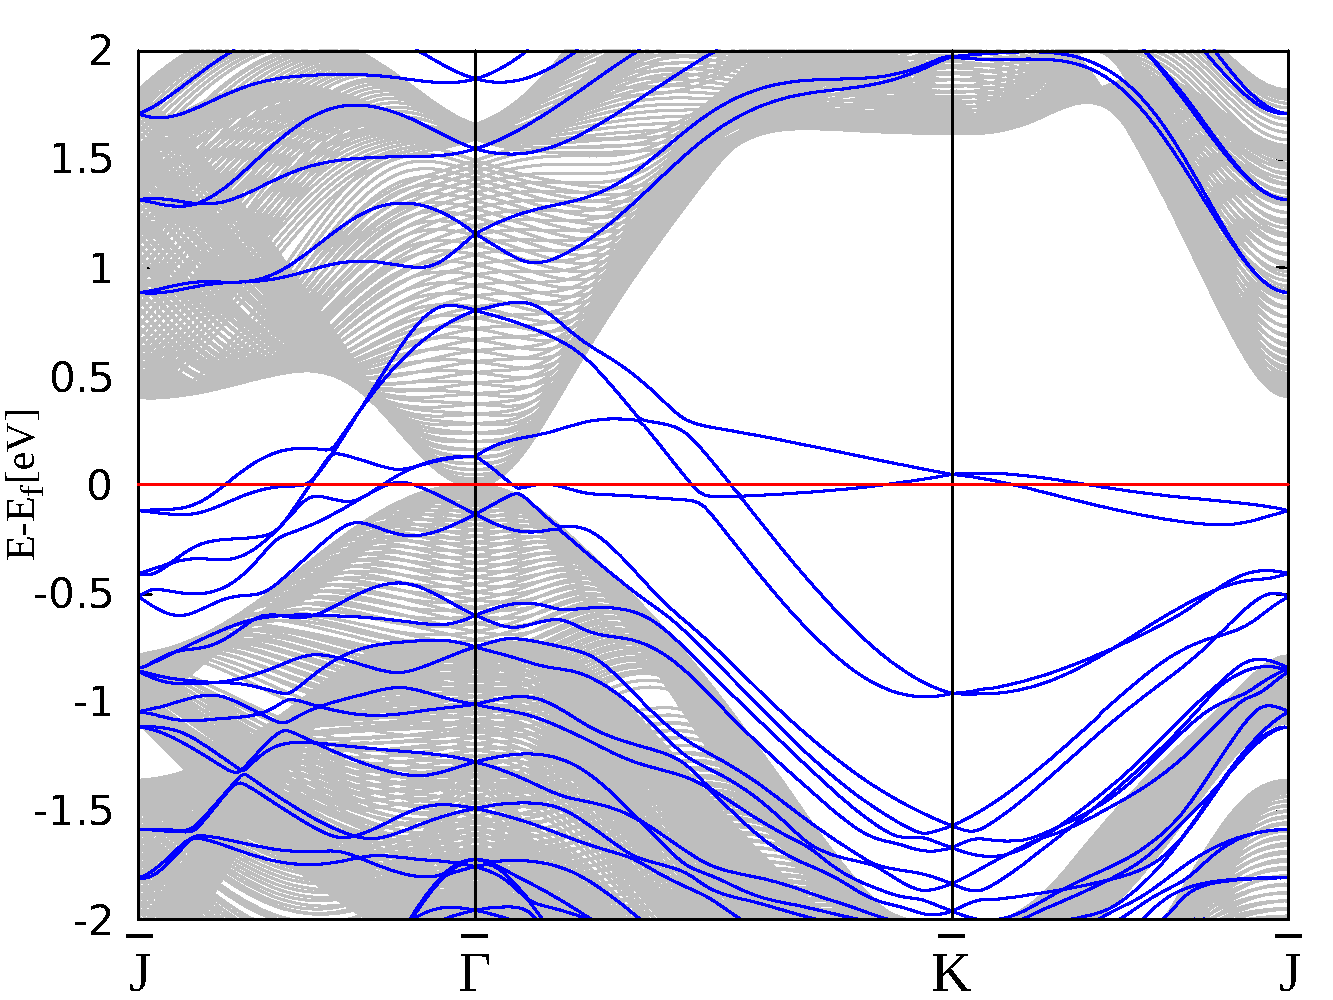
\includegraphics[width=\linewidth]{Hg_termination/bulk+9_layers_no_dos_-2_2.pdf}
%			\caption{9 layers with hydrogens on the bottom passivating one of the Hg surface terminations}
		\end{column}
	\end{columns}
	\vspace{.3cm}
	\footnotesize{
		First row: without hydrogens. \\Second row: with hydrogens passivating one surface.}
\end{frame}

\begin{frame}{PBBS with 16 and 17 layer slabs}
	\begin{columns}
		\begin{column}{.34\linewidth}
			\centering
			Te-Hg termination
		\end{column}
		\begin{column}{.34\linewidth}
			\centering
			Te-Te termination
		\end{column}
		\begin{column}{.34\linewidth}
			\centering
			Hg-Hg termination
		\end{column}
	\end{columns}
	\begin{columns}
		\begin{column}{.34\linewidth}
			\centering 
			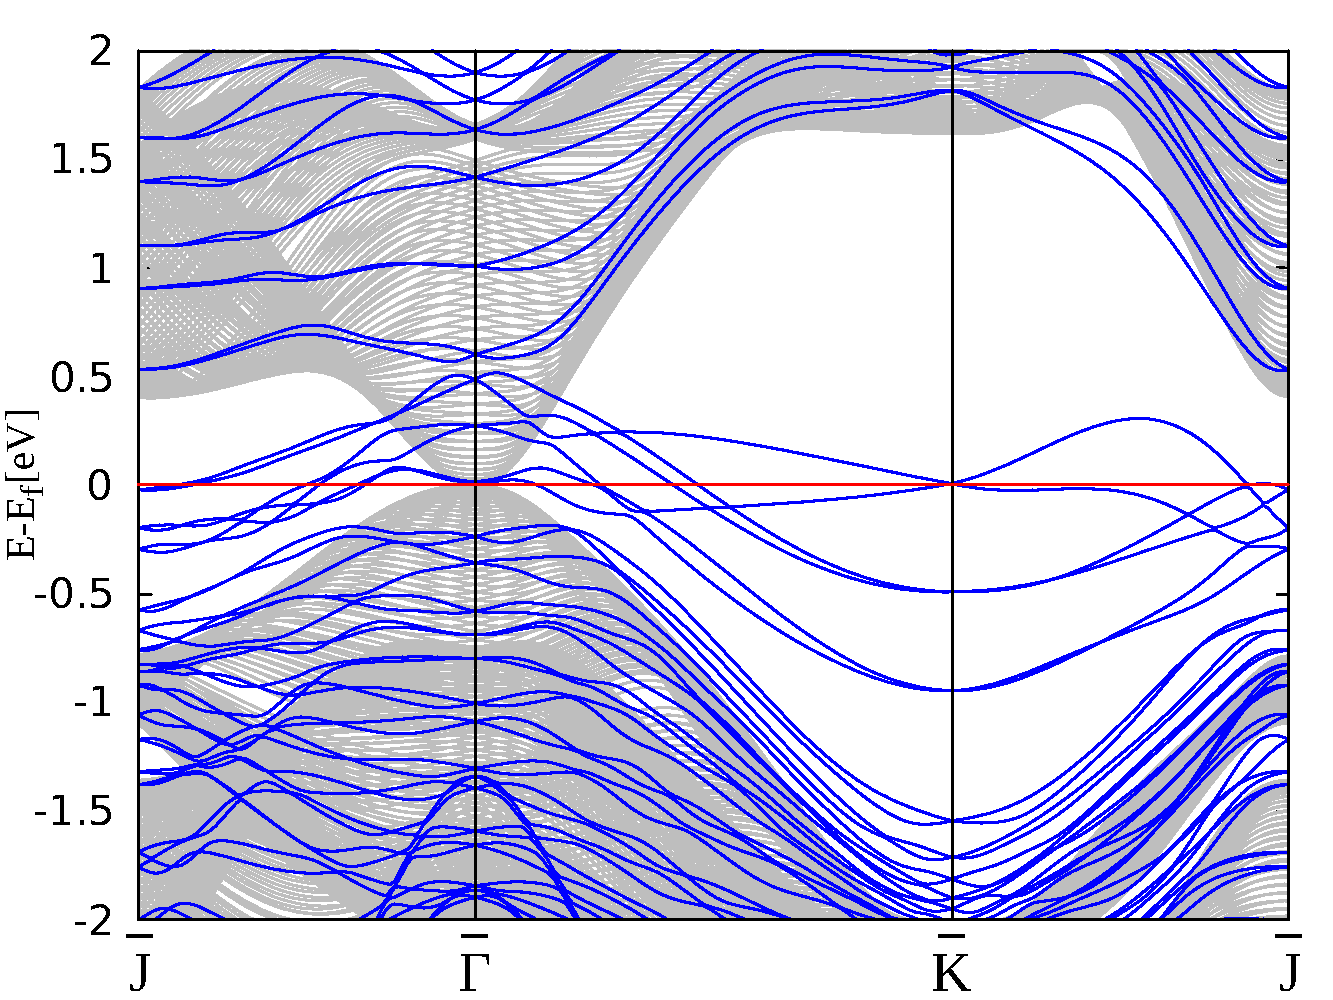
\includegraphics[width=\linewidth]{Te_and_Hg_termination/no_H_bulk+16_layers_no_dos_-2_2.pdf}
%			\caption{16 layers without hydrogens passivating the Te termination} \label{}
		\end{column}
		\begin{column}{.34\linewidth}
			\centering 
			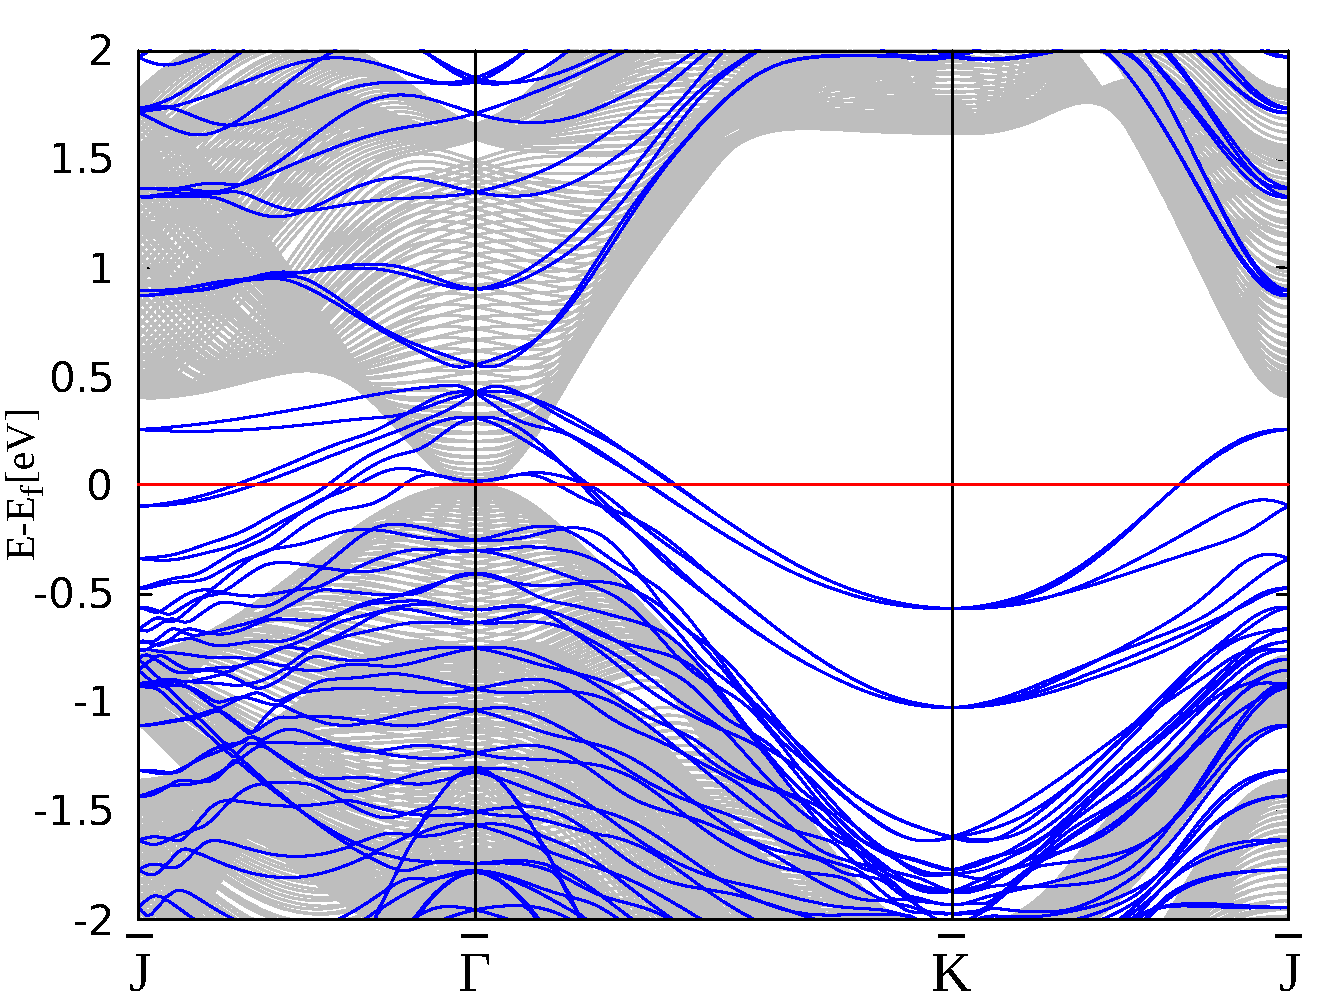
\includegraphics[width=\linewidth]{Te_termination/no_H_bulk+17_layers_no_dos_-2_2.pdf}
%			\caption{17 layers without hydrogens passivating one of the surfaces} 
		\end{column}
		\begin{column}{.34\linewidth}
			\centering 
			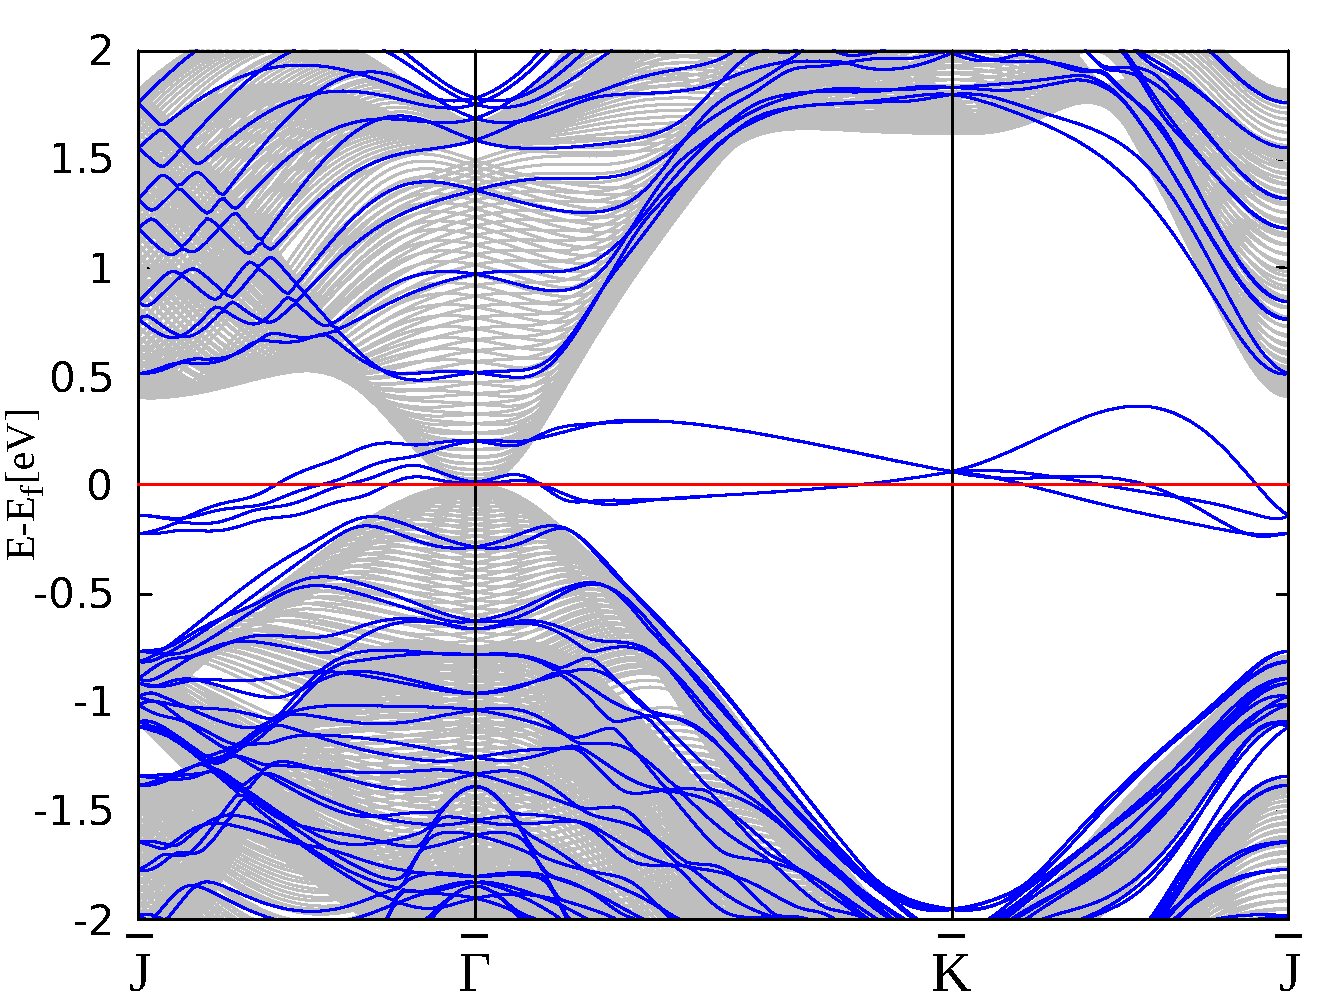
\includegraphics[width=\linewidth]{Hg_termination/no_H_bulk+17_layers_no_dos_-2_2.pdf}
%			\caption{17 layers without hydrogens passivating one of the surfaces} \label{}
		\end{column}
	\end{columns}
	\begin{columns}
		\begin{column}{.34\linewidth}
			\centering
			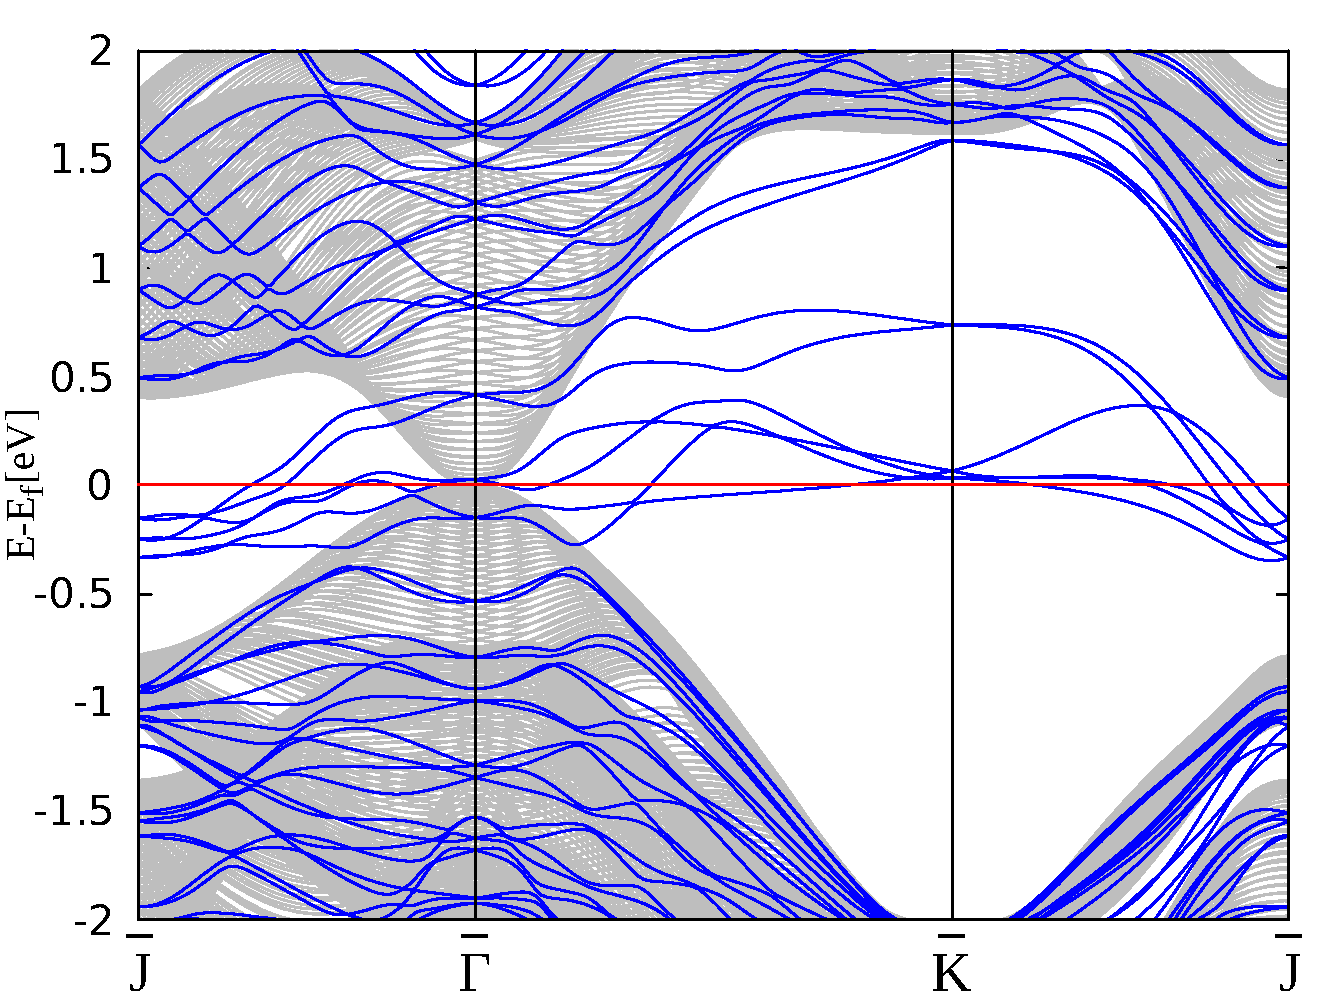
\includegraphics[width=\linewidth]{Te_and_Hg_termination/bulk+16_layers_no_dos_-2_2.pdf}
%			\caption{16 layers with hydrogens on the bottom passivating the Te surface terminations}
		\end{column}
		\begin{column}{.34\linewidth}
			\centering
			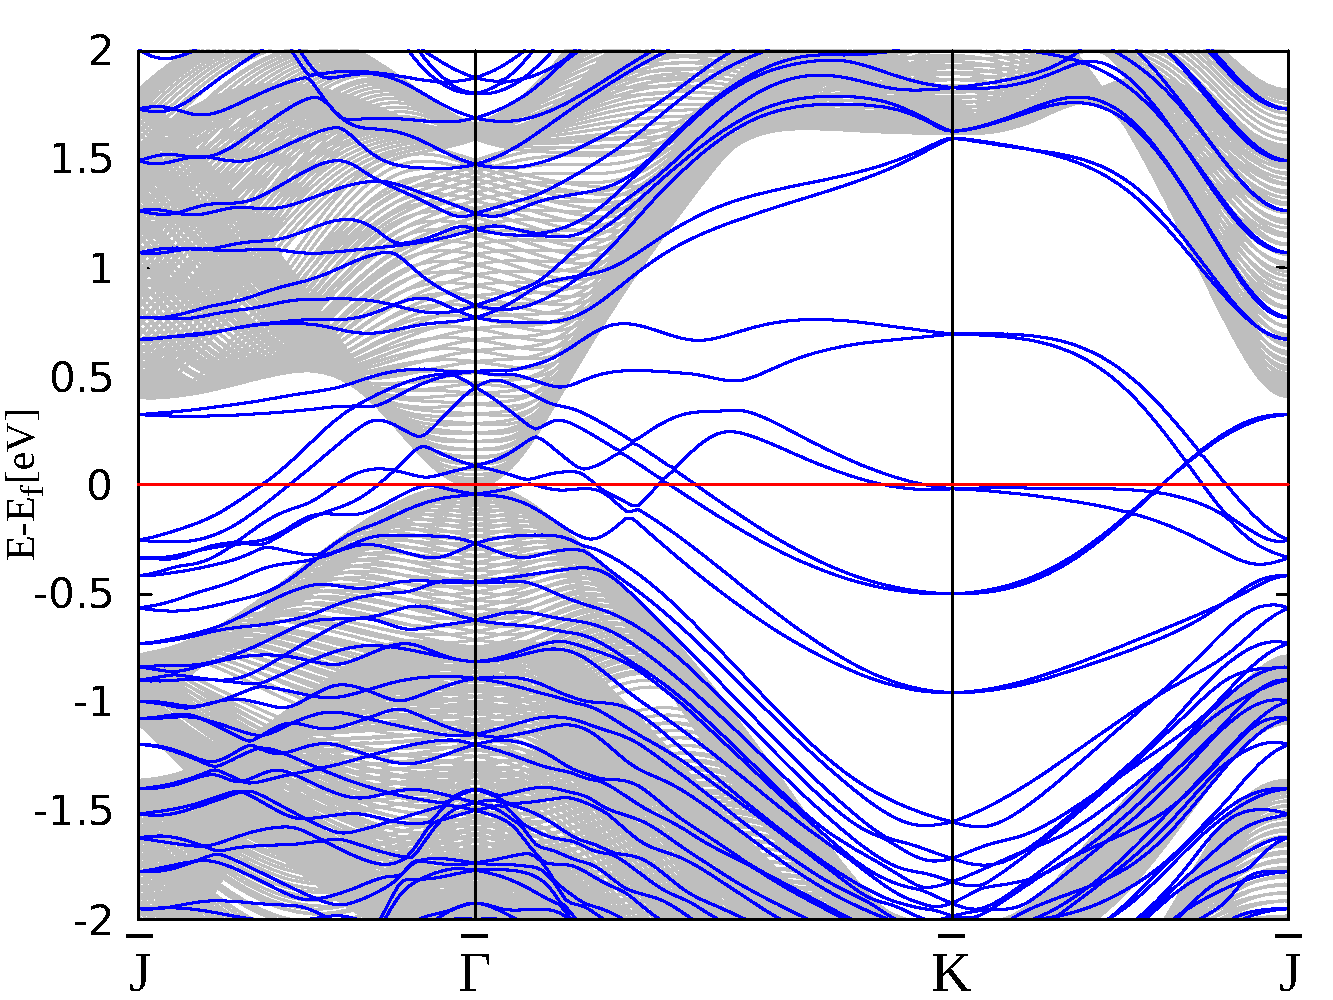
\includegraphics[width=\linewidth]{Te_termination/bulk+17_layers_no_dos_-2_2.pdf}
%			\caption{17 layers with hydrogens on the bottom passivating one of the Te surface terminations}
		\end{column}
		\begin{column}{.34\linewidth}
			\centering
			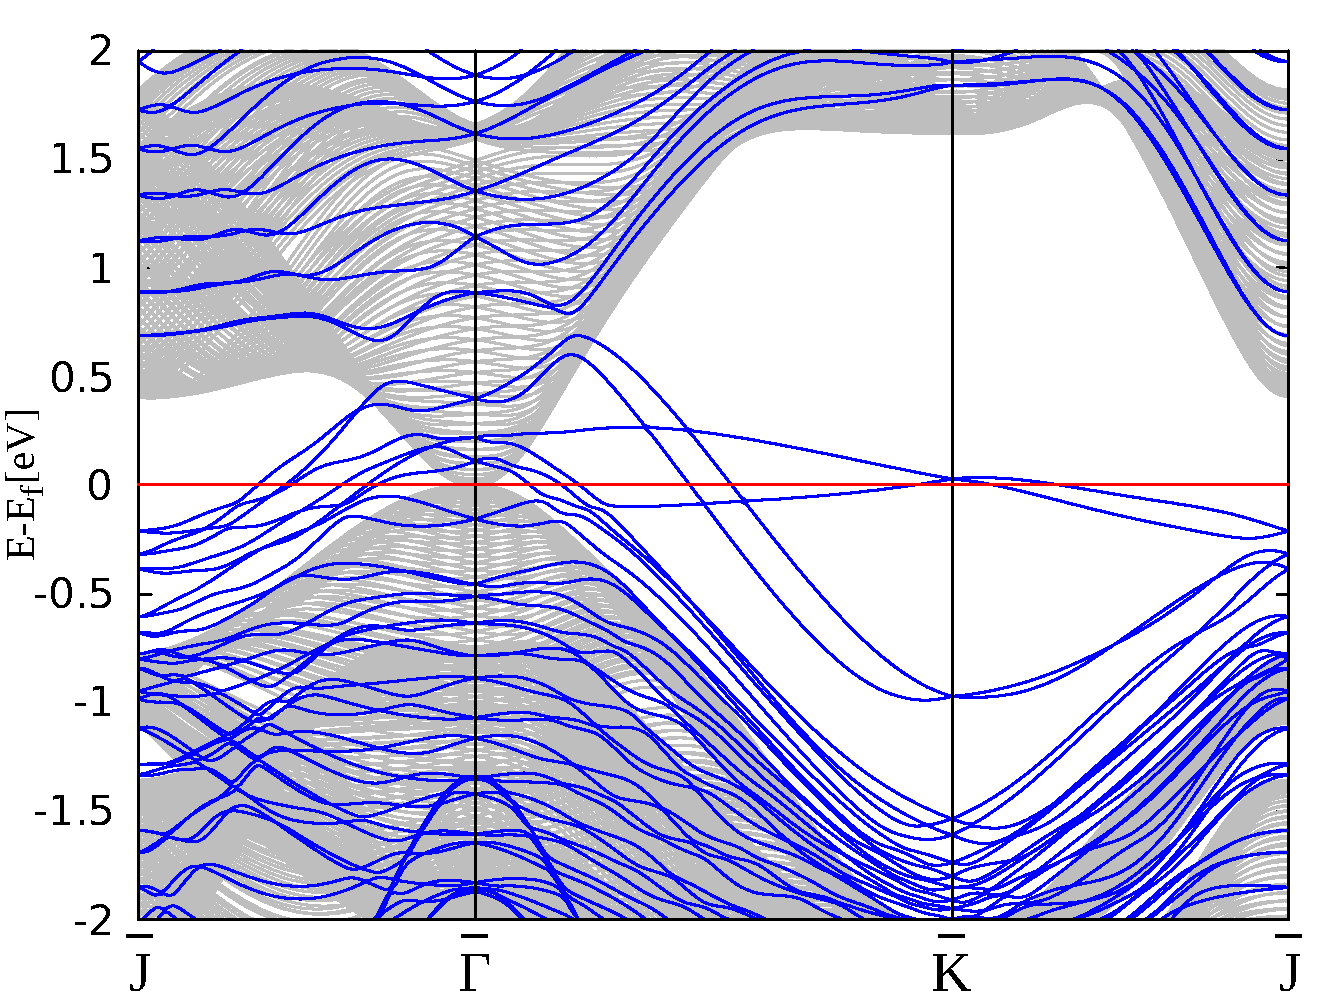
\includegraphics[width=\linewidth]{Hg_termination/bulk+17_layers_no_dos_-2_2.pdf}
%			\caption{17 layers with hydrogens on the bottom passivating one of the Hg surface terminations}
		\end{column}
	\end{columns}
	\vspace{.3cm}
	\footnotesize{
		First row: without hydrogens. \\Second row: with hydrogens passivating one surface.}
\end{frame}

%%% Local Variables:
%%% mode: latex
%%% TeX-master: "main_BA2_Vortrag.tex"
%%% End: